\section{Signal region, control region, and sideband definitions}
\label{sec:region_definitions}

Several regions of phase space are explored in the analysis. The signal region is accompanied by \glspl{CR} and \glspl{SB} to aid in the prediction of certain backgrounds, as explained below. The preselection is applied to every region, so they are separated by the \acrshort{cms} datasets used, the \acrlong{hlt} requirements, and object and/or kinematic selections.

% This section is up-to-date as of 12th August


%=========================================================


\subsection{The signal region}
\label{subsec:htoinv_signal_region}

The signal region is the area of parameter space where we expect the signal to manifest, and the background to be reduced sufficiently that the potential presence of signal in data can be statistically verified. In this analysis, only hadronic final states are permitted. Events with leptons, photons and taus meeting the loose or veto criteria in Chpt.~\ref{sec:analysis_objects} are vetoed.

Events must satisfy a logical or of \acrshort{hlt} cross-triggers for \acrlong{pf} \ptmiss and \mht calculated without muons,\footnote{Why/how exactly is this done? Can muons fake jets, and so these calculations omit muons matched to jets at PF/HLT level?} and at least one \gls{jet} fulfilling the tight ID criteria (see Chpt.~\ref{sec:analysis_objects}). The triggers are illustrated in Tab.~\ref{tab:htoinv_SR_triggers}.

\begin{table}[htbp]
    \centering
    \begin{tabular}{ccccc}
        \hline\hline
        Year & $\ptmissNoMu$ (\GeVns) & $\mhtNoMu$ (\GeVns) & $\HT$ (\GeVns) & $\njet$ with tight ID \\ \hline
        \multirow{4}{*}{2016} & 90 & 90 & --- & $\geq \text{1}$ \\
        & 100 & 100 & --- & $\geq \text{1}$ \\
        & 110 & 110 & --- & $\geq \text{1}$ \\
        & 120 & 120 & --- & $\geq \text{1}$ \\
        \hline
        \multirow{2}{*}{2017} & 120 & 120 & --- & $\geq \text{1}$ \\
        & 120 & 120 & 60 & $\geq \text{1}$ \\
        \hline
        2018 & 120 & 120 & --- & $\geq \text{1}$ \\
        \hline\hline
    \end{tabular}
    \caption[The trigger thresholds required for events to enter the signal region in each data taking year]{The trigger thresholds required for events to enter the signal region in each data taking year. Each quantity is computed with the \gls{particleflow} at \acrshort{hlt} level. The variables \ptmiss and \mht do not include muons in the calculations.}
    \label{tab:htoinv_SR_triggers}
\end{table}

The \ptmiss distribution from simulation in the signal region after the analysis-level selection are shown for the \ttH and \VH resolved and boosted categories in Fig.~\ref{fig:htoinv_sr_yields_comb2016to18}. Event yields are scaled to the integrated luminosity of the full Run-2 dataset.

\begin{figure}[htbp]
    \centering
    \begin{subfigure}[b]{0.24\textwidth}
        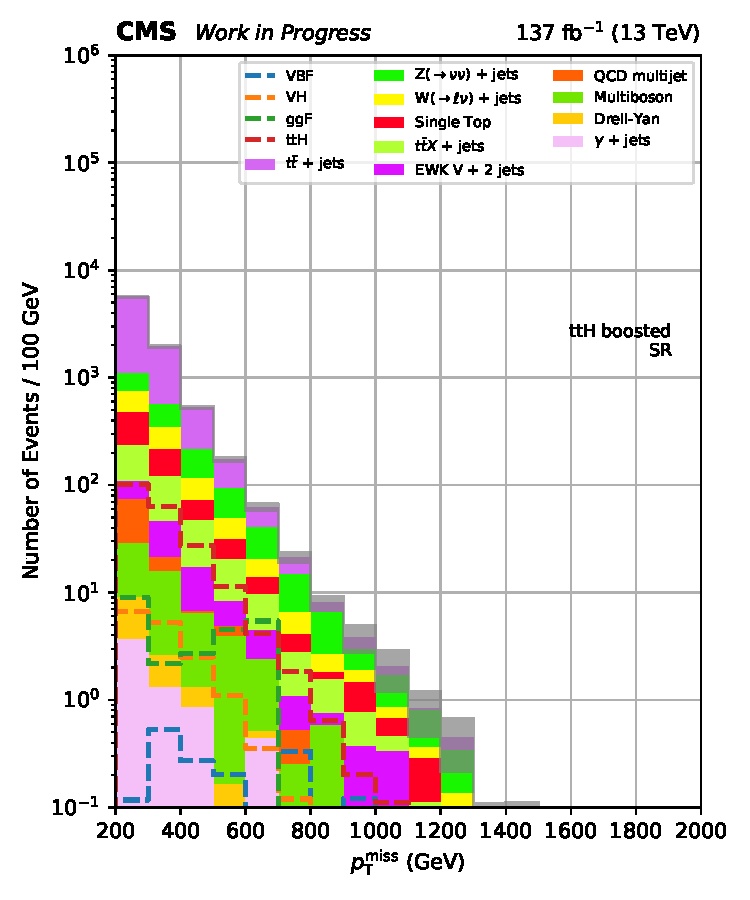
\includegraphics[width=\textwidth]{figures/region_plots/full_Run2/region_0/ttH_boosted.pdf}
        \caption{\ttH boosted}
    \end{subfigure}
    \hfill
    \begin{subfigure}[b]{0.24\textwidth}
        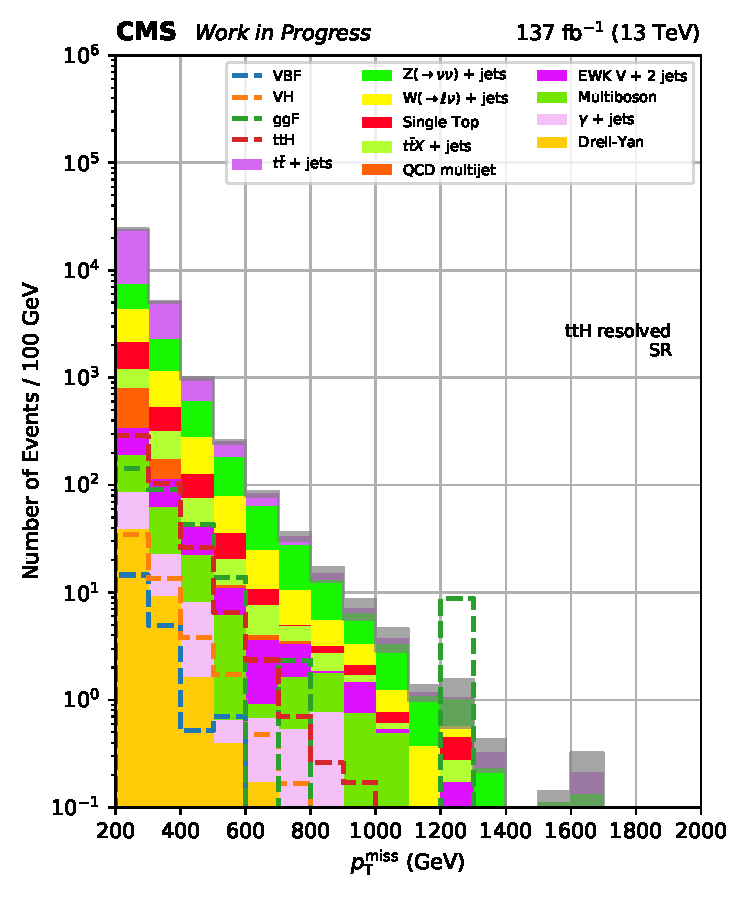
\includegraphics[width=\textwidth]{figures/region_plots/full_Run2/region_0/ttH_resolved.pdf}
        \caption{\ttH resolved}
    \end{subfigure}
    \begin{subfigure}[b]{0.24\textwidth}
        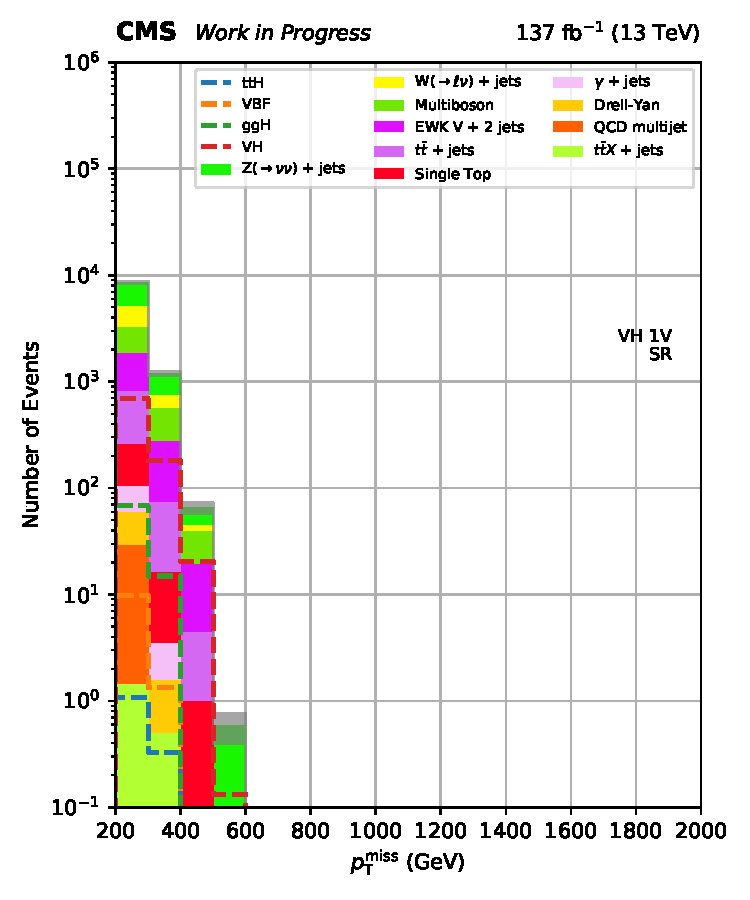
\includegraphics[width=\textwidth]{figures/region_plots/full_Run2/region_0/VH_1V.pdf}
        \caption{\VH 1V}
    \end{subfigure}
    \hfill
    \begin{subfigure}[b]{0.24\textwidth}
        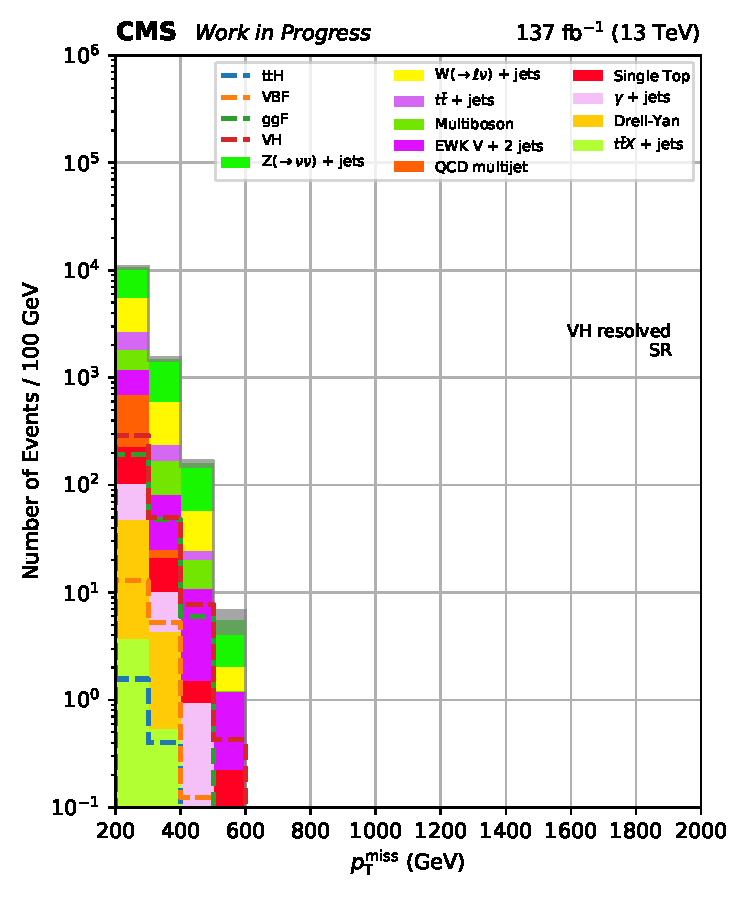
\includegraphics[width=\textwidth]{figures/region_plots/full_Run2/region_0/VH_resolved.pdf}
        \caption{\VH resolved}
    \end{subfigure}
    \caption[Data-simulation comparisons of the \ptmiss distribution in the signal region for the combined boosted and resolved categories for the \ttH and \VH processes, using simulation derived for each year in Run-2 and scaled to the required luminosity]{Data-simulation comparisons of the \ptmiss distribution in the signal region for the combined boosted and resolved categories for the \ttH and \VH processes, using simulation derived for each year in Run-2 and scaled to the required luminosity.}
    \label{fig:htoinv_sr_yields_comb2016to18}
\end{figure}

% Figures from 2nd September, 2020


%=========================================================


\subsection{Control regions}
\label{subsec:htoinv_control_regions}

\Glspl{CR} serve two complementary purposes in many analyses: the prediction of certain backgrounds that dominate in the signal region, as a more accurate method than using the yields directly from \acrlong{mc}; and to validate the data, \acrshort{mc}, and corrections or weights applied. They are orthogonal to the signal region and to each other by way of lepton or photon requirements, and by triggers that may pertain to those objects. \Glspl{CR} are also designed to, ideally, be devoid of signal. Contamination is sometimes present, but at a very small level. Five \glspl{CR} are used in the analysis: \singleMuCr \doubleMuCr, \singleEleCr \doubleEleCr, and \singlePhotonCr. The criteria for the objects---which are defined explicitly in Chpt.~\ref{sec:analysis_objects}---are summarised in the list below.
\medskip
\begin{easylist}[itemize]
    \easylistprops
    & \singleMuCr: one tight muon \tightMuon with $\pt > \text{20}\GeV$ and a transverse mass (as calculated in Eq.~\ref{eq:transverse_mass_massless}) in the range $\text{50} < \mtMuon < \text{110}\GeV$
    & \doubleMuCr: one tight muon \tightMuon with $\pt > \text{20}\GeV$, and one loose muon \looseMuon with $\pt > \text{10}\GeV$ that has opposite charge, with a combined invariant mass of $\text{60} < \doubleMuMass < \text{120}\GeV$ in the \VH and \ggH subcategories, while instead $\text{75} < \doubleMuMass < \text{105}\GeV$ in the \ttH subcategories. The leading muon (regardless of whether it is the tight or loose one) is required to possess $\pt > \text{110}\GeV$
    & \singleEleCr: one tight electron \tightEle with $\pt > \text{40}\GeV$ and $\text{50} < \mtElectron < \text{110}\GeV$
    & \doubleEleCr: one tight electron \tightEle with $\pt > \text{40}\GeV$, and one veto electron \vetoEle with $\pt > \text{10}\GeV$ that has opposite charge, with a combined invariant mass of $\text{60} < \doubleEleMass < \text{120}\GeV$ in the \VH and \ggH subcategories, while instead $\text{75} < \doubleEleMass < \text{105}\GeV$ in the \ttH subcategories. The leading electron (regardless of whether it is the tight or loose one) is required to possess $\pt > \text{110}\GeV$
    & \singlePhotonCr: one medium photon \mediumPhoton with $\pt > \text{230}\GeV$
\end{easylist}

\medskip

\noindent{}The transverse mass cuts in the single lepton \glspl{CR} reduce the effect of signal contamination, specifically from \ttH since its \mT generally eclipses that of \ttbar.\footnote{The \mT for a \ttbar event with \ptvecmiss solely from the neutrino (in $\HepProcess{\Ptop \to \Pbottom\PW}$, $\HepProcess{\PW \to \Plepton\Pnu}$) should be in a window around the \PW mass. Introducing additional decay products such as the Higgs boson increase it.} The trigger requirements for the \singleMuCr and \doubleMuCr \glspl{CR} are the same as for the signal region (Tab.~\ref{tab:htoinv_SR_triggers}) since the same primary dataset is used.\footnote{If we decide to go ahead, mention somewhere that the angular variable cuts in the categorisation table are not applied in the control regions to improve stats. The MET shapes were found to be consistent if they were applied vs. not applied. And the expected limit from a CR-only fit improved across the board when removed.}

In the \doubleMuCr and \doubleEleCr \glspl{CR}, the \doubleLepMass window is halved for the \ttH subcategories compared to the others to reduce contamination from \ttbar, granting a a higher purity \ztolplmpjets region. The leading lepton \pt requirement is increased in these regions for all categories also for purity purposes.

The \singleEleCr and \doubleEleCr \glspl{CR} take advantage of the increased statistical power of two primary datasets in both 2016 and 2017, characterised by electron and photon triggers. In 2018, they were merged into a single $\Pe/\Pphoton$ primary dataset. Tabs.~\ref{tab:htoinv_ele_pd_triggers} and~\ref{tab:htoinv_photon_pd_triggers} elucidate how the trigger requirements are specified for each year. As before, each quantity and object is defined at \acrshort{hlt} level. If an event aims to enter the \singleEleCr or \doubleEleCr, and is from the dataset of \Pe-based triggers, the criteria for either of the two triggers for the given year in Tab.~\ref{tab:htoinv_ele_pd_triggers} must be satisfied. If an event aims to enter either \gls{CR} and is from the primary dataset of \Pphoton-based triggers, the failure of both of the electron triggers in Tab.~\ref{tab:htoinv_ele_pd_triggers} and the passing of any of the photon triggers in Tab.~\ref{tab:htoinv_photon_pd_triggers} are required. This condition avoids double counting events that also appear in the electron trigger-based dataset. In 2018, any of the year's triggers in Tabs.~\ref{tab:htoinv_ele_pd_triggers} and~\ref{tab:htoinv_photon_pd_triggers} may be satisfied. For \acrlong{mc} events, as they are not categorised by trigger, they may pass any of the triggers in either table for their respective year.\footnote{See if I can describe the trigger requirements in a more elegant way. Might be easier give the descriptions and actual HLT path names a bit earlier, then just reference the HLT path names in the list.}

\begin{table}[htbp]
    \centering
    \begin{tabular}{ccccc}
        \hline\hline
        Year & $E_{\mathrm{T}, \,\mathrm{SC}}^{\Pe}$ threshold (\GeVns) & \Pe WP & Calorimeter ID & \acrshort{gsf} track-SC matching \\ \hline
        \multirow{2}{*}{2016} & 27 & Tight & --- & --- \\
        & 105 & --- & Very tight & Tight \\\hline
        \multirow{2}{*}{2017} & 35 & Tight & --- & --- \\
        & 115 & --- & Very tight & Tight \\\hline
        \multirow{2}{*}{2018} & 32 & Tight & --- & --- \\
        & 115 & --- & Very tight & Tight \\
        \hline\hline
    \end{tabular}
    \caption[The trigger requirements for events to enter the \singleEleCr or \doubleEleCr control regions, if they originate from the dataset of \Pe-based triggers]{The trigger requirements for events to enter the \singleEleCr or \doubleEleCr \glspl{CR}, if they originate from the dataset of \Pe-based triggers. Selections are on the transverse energy of the supercluster $E_{\mathrm{T}, \,\mathrm{SC}}$, the working point of the candidate electron, ID of the candidate in the calorimeters, and the matching between the \acrfull{gsf}-fitted track and supercluster, all at \acrshort{hlt} level.}
    \label{tab:htoinv_ele_pd_triggers}
\end{table}

For the \singlePhotonCr \gls{CR}, we take data from \acrshort{cms} originating only from the dataset of \Pphoton-based triggers. Data and \acrshort{mc} must satisfy any of the triggers from Tab.~\ref{tab:htoinv_photon_pd_triggers} for the respective year.

\begin{table}[htbp]
    \centering
    \begin{tabular}{ccc}
        \hline\hline
        Year & $\ET^{\Pphoton}$ threshold (\GeVns) & $H/E$ \\\hline
        \multirow{2}{*}{2016} & 165 & $< \text{0.1}$ \\
        & 175 & --- \\\hline
        2017 & 200 & --- \\\hline
        2018 & 200 & --- \\\hline\hline
    \end{tabular}
    \caption[The trigger requirements for events to enter the \singleEleCr \doubleEleCr, or \singlePhotonCr control regions, if they originate from the dataset of \Pphoton-based triggers]{The trigger requirements for events to enter the \singleEleCr \doubleEleCr, or \singlePhotonCr \gls{CR}, if they originate from the dataset of \Pphoton-based triggers. Selections are on the transverse energy \ET of the candidate, and the ratio of the candidate's central energy deposit in the \acrshort{hcal} to the \acrshort{ecal} ($H/E$), all computed at \acrshort{hlt} level.}
    \label{tab:htoinv_photon_pd_triggers}
\end{table}

In each of the \glspl{CR}, the \ptvecmiss is recalculated without the objects used to define said region to model the process it is predicting. In essence, these objects are treated as a source of missing momentum. Conditions in the event selection and binning that refer to \ptmiss use the recalculated quantity when applied to the \glspl{CR}. Using the \singleMuCr \gls{CR} as an example, the new \ptvecmiss is the vector sum of the old \ptvecmiss and the tight muon \ptvec. The single lepton \glspl{CR} estimate the semi-leptonic $\ttbarpjets$ and $\wtolnupjets$ backgrounds. In both cases, they may enter the signal region if the lepton is lost, becoming a source of \ptmiss. The dilepton and \singlePhotonCr regions consider \ztonunupjets. The former parallels the decay as it is enriched in \ztolplmpjets---possessing very similar kinematic properties while being much easier to detect, improving statistical accuracy. The latter region substitutes the \ztonunu decay with a photon.

Figs.~\ref{fig:htoinv_cr_yields_comb2016to18_single_muon}, \ref{fig:htoinv_cr_yields_comb2016to18_double_muon}, \ref{fig:htoinv_cr_yields_comb2016to18_single_electron}, \ref{fig:htoinv_cr_yields_comb2016to18_double_electron}, and \ref{fig:htoinv_cr_yields_comb2016to18_single_photon} reveal the \ptmiss distributions in each \gls{CR} after the analysis-level selections with the full Run-2 dataset. The combined \ttH and \VH subcategories for boosted and resolved topologies are used to demonstrate the shapes and data--simulation agreement. Background estimation is performed separately for each year due to the differing running conditions, detector configuration, and the different effects or problems seen in the data.\footnote{Might not need to show all of these plots. They're just here for now, and can be tidied up later. May be worth showing \ggH in the same capacity as the other categories, however.}

\begin{figure}[htbp]
    \centering
    \begin{subfigure}[b]{0.24\textwidth}
        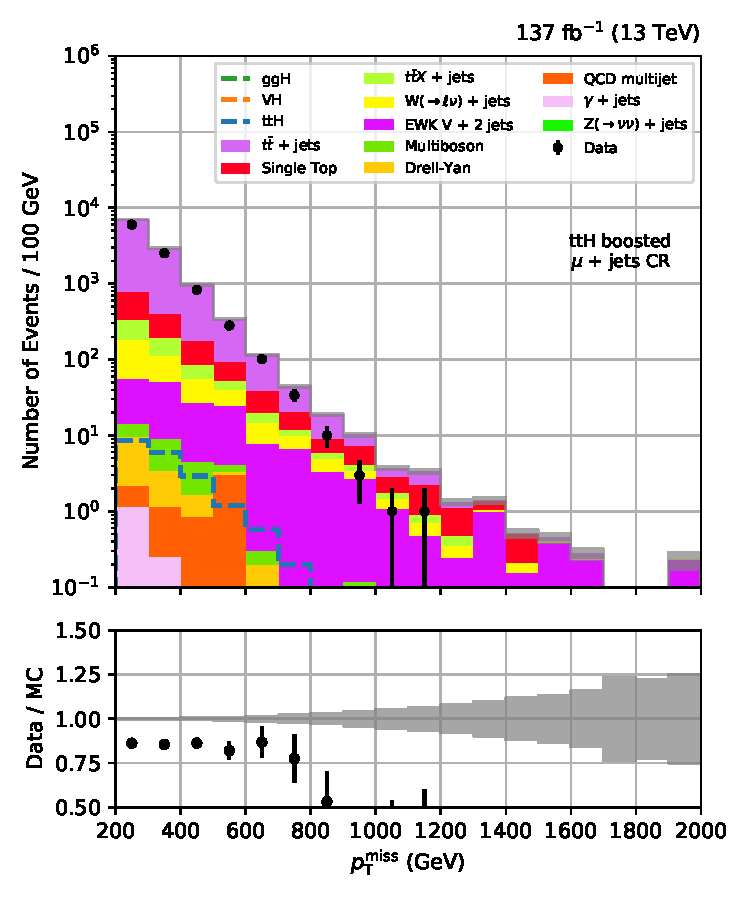
\includegraphics[width=\textwidth]{figures/region_plots/full_Run2/region_1/ttH_boosted.pdf}
        \caption{\ttH boosted}
    \end{subfigure}
    \hfill
    \begin{subfigure}[b]{0.24\textwidth}
        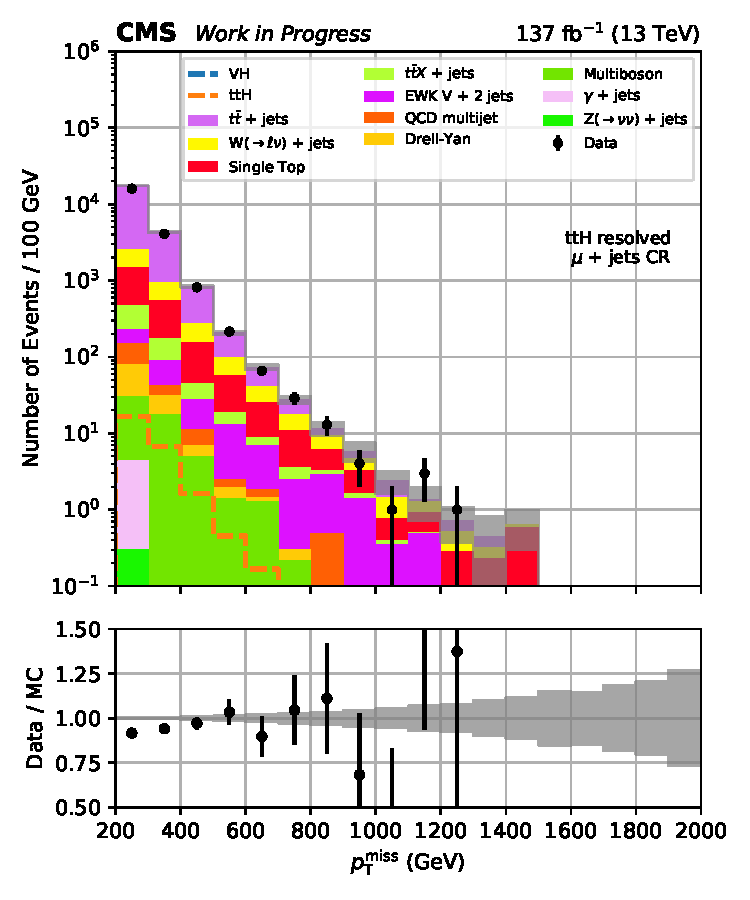
\includegraphics[width=\textwidth]{figures/region_plots/full_Run2/region_1/ttH_resolved.pdf}
        \caption{\ttH resolved}
    \end{subfigure}
    \hfill
    \begin{subfigure}[b]{0.24\textwidth}
        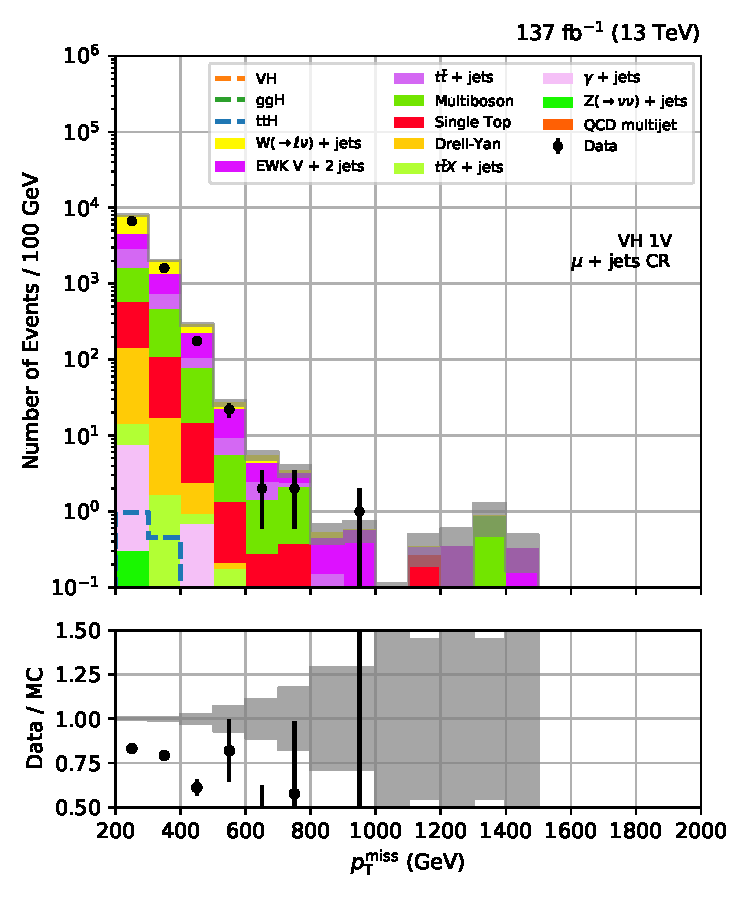
\includegraphics[width=\textwidth]{figures/region_plots/full_Run2/region_1/VH_1V.pdf}
        \caption{\VH 1V}
    \end{subfigure}
    \hfill
    \begin{subfigure}[b]{0.24\textwidth}
        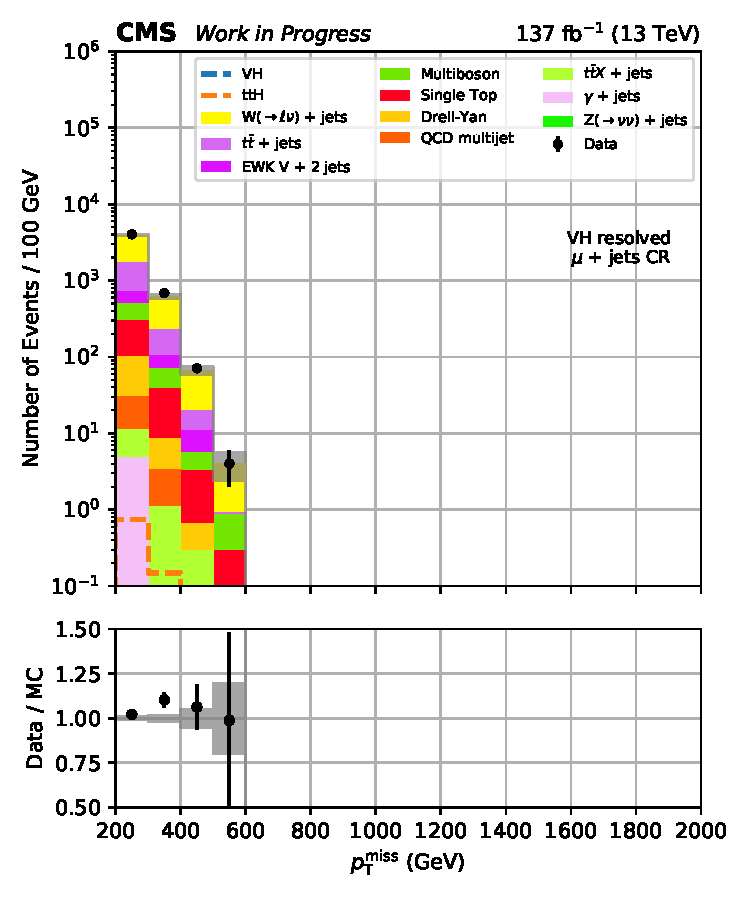
\includegraphics[width=\textwidth]{figures/region_plots/full_Run2/region_1/VH_resolved.pdf}
        \caption{\VH resolved}
    \end{subfigure}
    \caption[Data-simulation comparisons of the \ptmiss distribution in the \singleMuCr control region for the combined boosted and resolved categories for the \ttH and \VH processes, using the full Run-2 dataset]{Data-simulation comparisons of the \ptmiss distribution in the \singleMuCr \gls{CR} for the combined boosted and resolved categories for the \ttH and \VH processes, using the full Run-2 dataset.}
    \label{fig:htoinv_cr_yields_comb2016to18_single_muon}
\end{figure}

\begin{figure}[htbp]
    \centering
    \begin{subfigure}[b]{0.24\textwidth}
        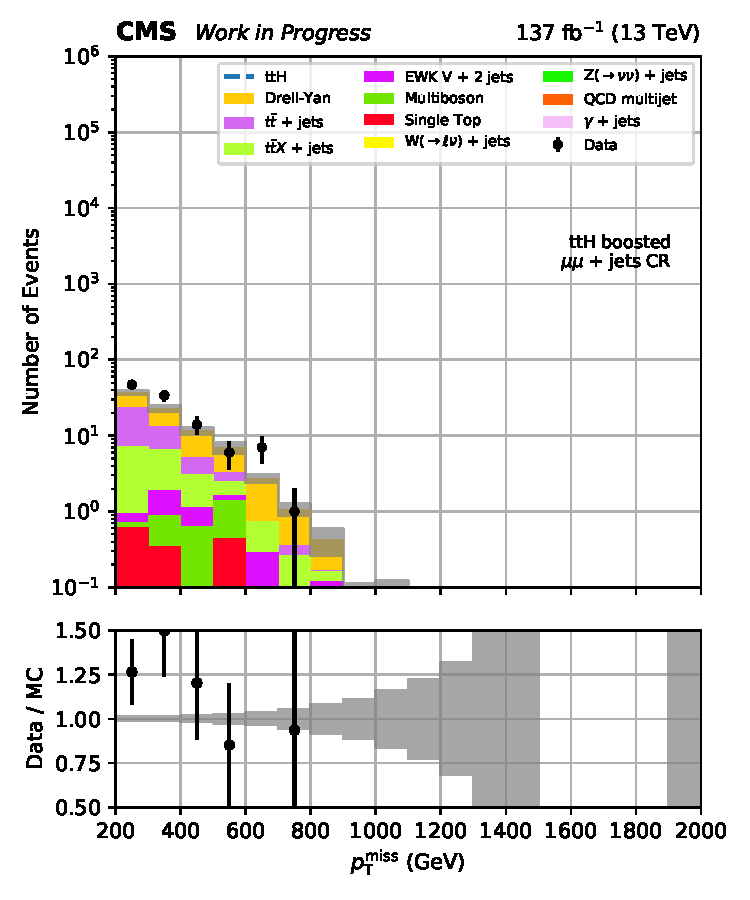
\includegraphics[width=\textwidth]{figures/region_plots/full_Run2/region_2/ttH_boosted.pdf}
        \caption{\ttH boosted}
    \end{subfigure}
    \hfill
    \begin{subfigure}[b]{0.24\textwidth}
        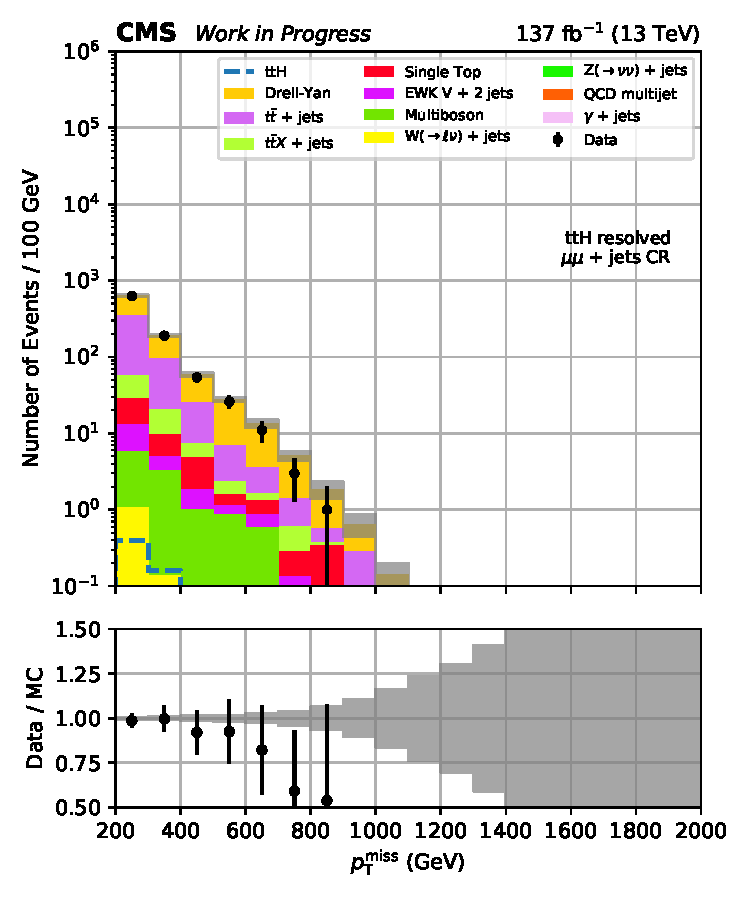
\includegraphics[width=\textwidth]{figures/region_plots/full_Run2/region_2/ttH_resolved.pdf}
        \caption{\ttH resolved}
    \end{subfigure}
    \hfill
    \begin{subfigure}[b]{0.24\textwidth}
        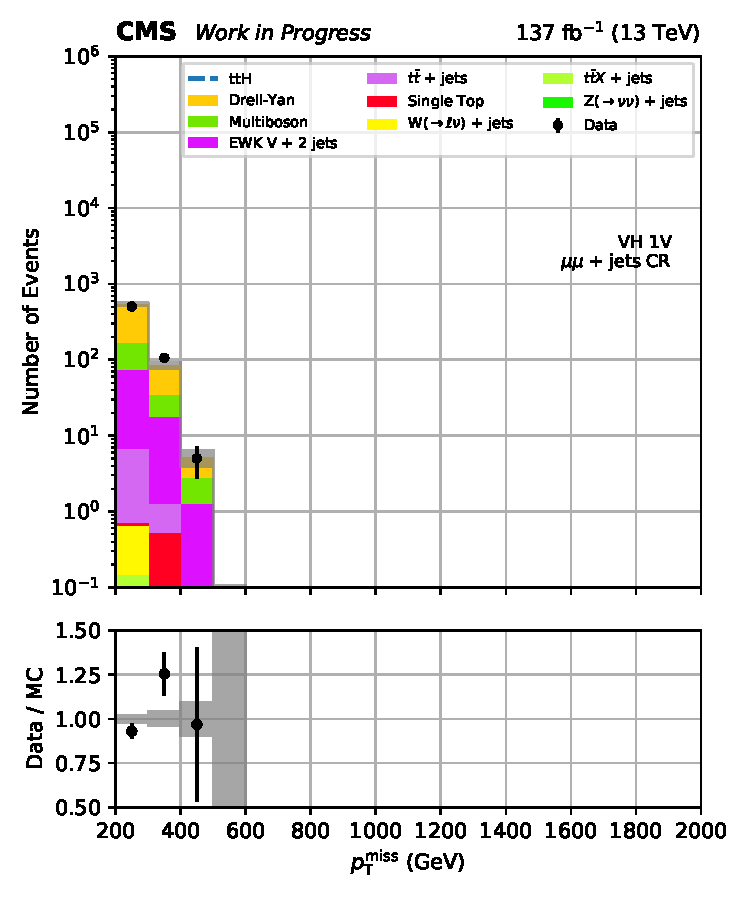
\includegraphics[width=\textwidth]{figures/region_plots/full_Run2/region_2/VH_1V.pdf}
        \caption{\VH 1V}
    \end{subfigure}
    \hfill
    \begin{subfigure}[b]{0.24\textwidth}
        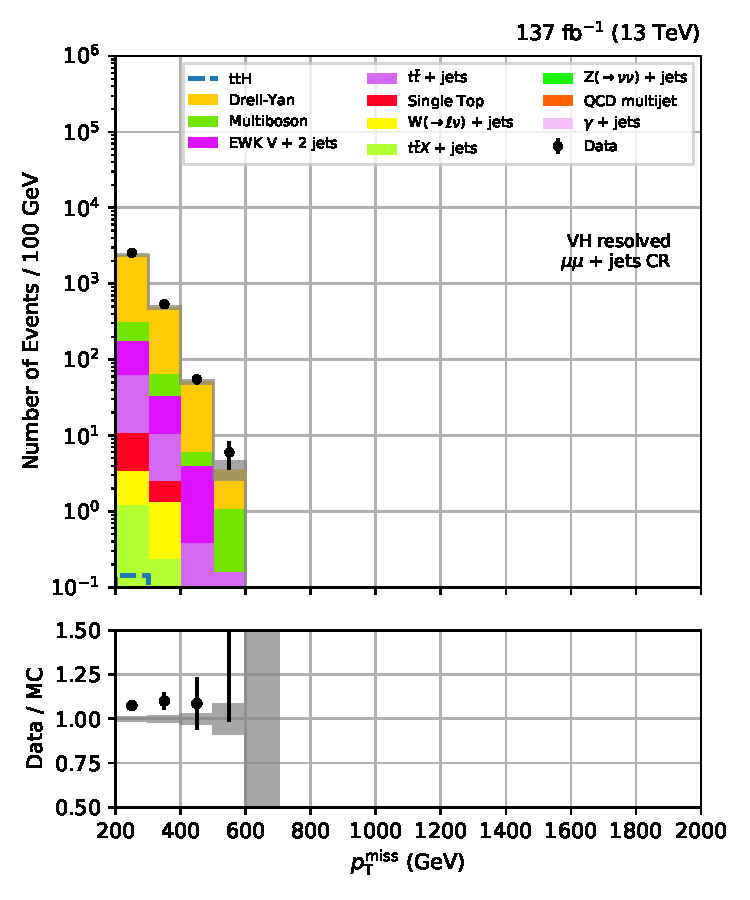
\includegraphics[width=\textwidth]{figures/region_plots/full_Run2/region_2/VH_resolved.pdf}
        \caption{\VH resolved}
    \end{subfigure}
    \caption[Data-simulation comparisons of the \ptmiss distribution in the \doubleMuCr control region for the combined boosted and resolved categories for the \ttH and \VH processes, using the full Run-2 dataset]{Data-simulation comparisons of the \ptmiss distribution in the \doubleMuCr \gls{CR} for the combined boosted and resolved categories for the \ttH and \VH processes, using the full Run-2 dataset.}
    \label{fig:htoinv_cr_yields_comb2016to18_double_muon}
\end{figure}

\begin{figure}[htbp]
    \centering
    \begin{subfigure}[b]{0.24\textwidth}
        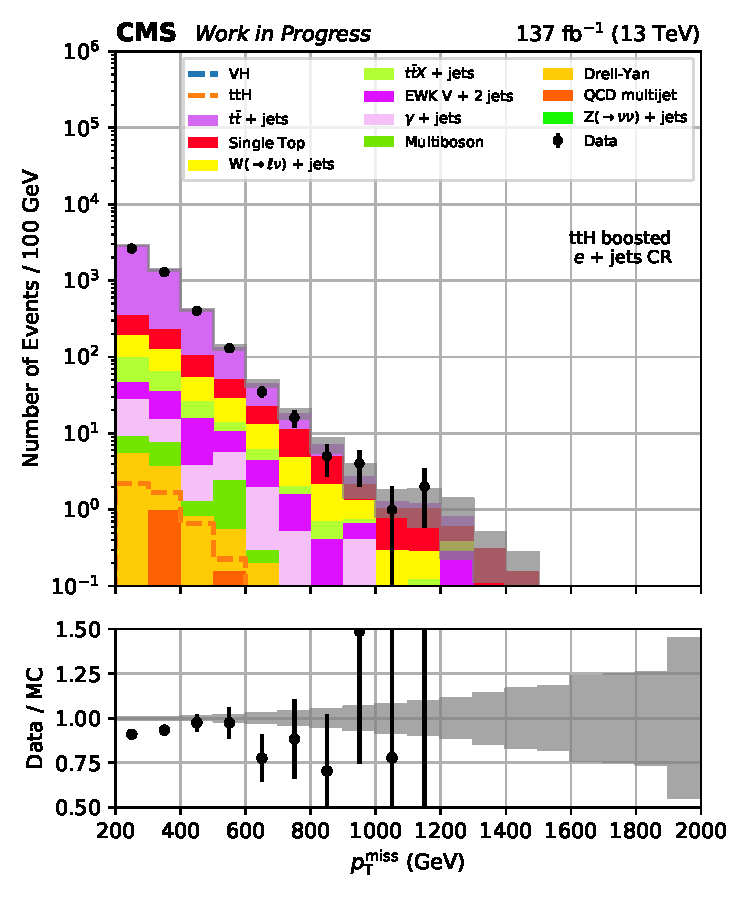
\includegraphics[width=\textwidth]{figures/region_plots/full_Run2/region_3/ttH_boosted.pdf}
        \caption{\ttH boosted}
    \end{subfigure}
    \hfill
    \begin{subfigure}[b]{0.24\textwidth}
        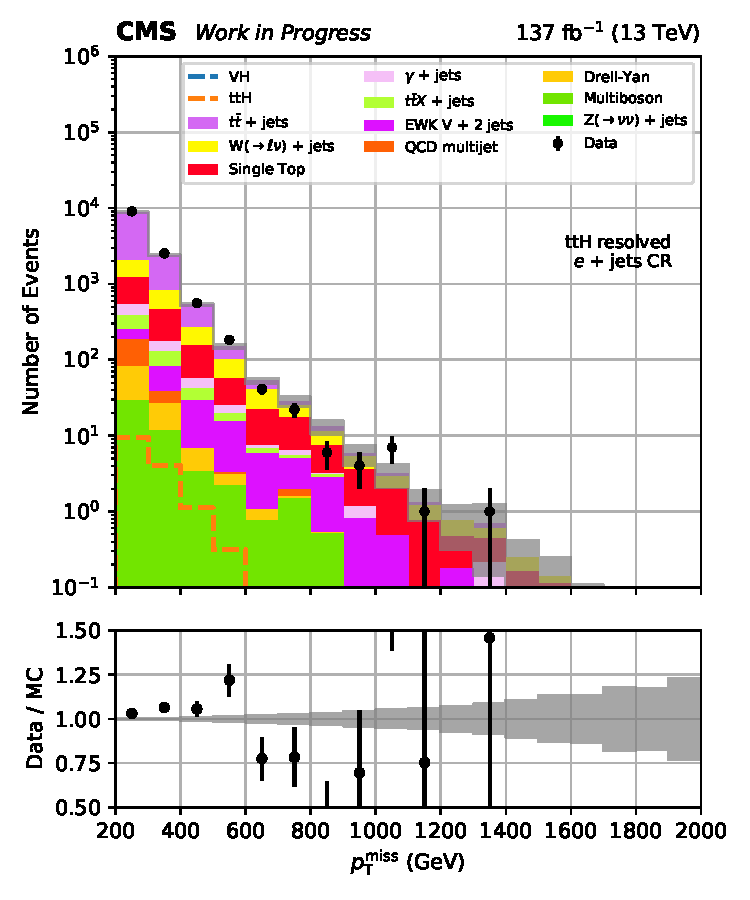
\includegraphics[width=\textwidth]{figures/region_plots/full_Run2/region_3/ttH_resolved.pdf}
        \caption{\ttH resolved}
    \end{subfigure}
    \hfill
    \begin{subfigure}[b]{0.24\textwidth}
        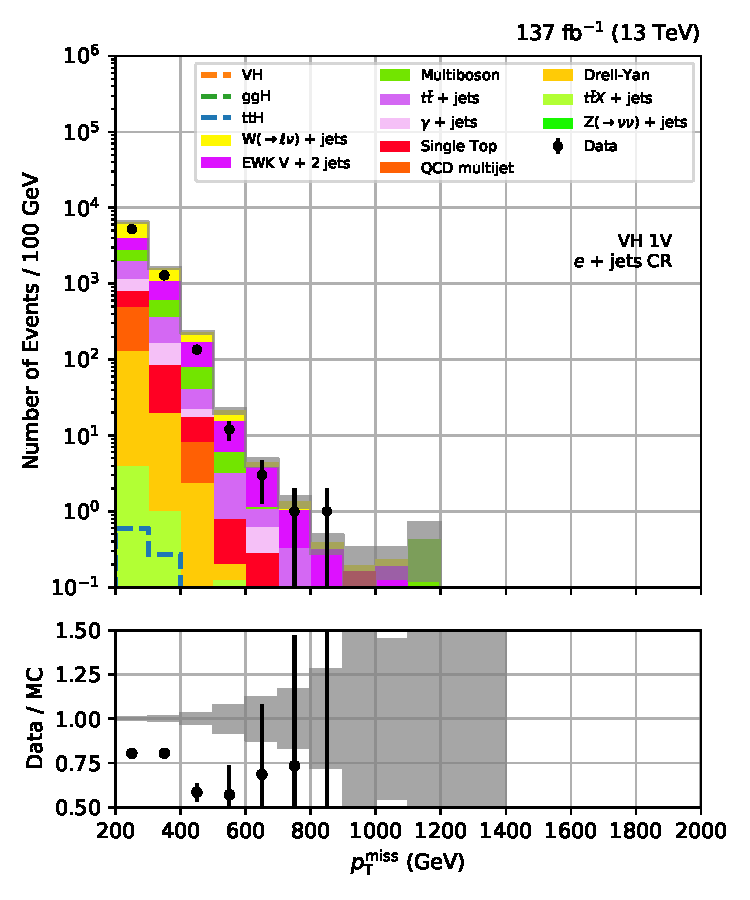
\includegraphics[width=\textwidth]{figures/region_plots/full_Run2/region_3/VH_1V.pdf}
        \caption{\VH 1V}
    \end{subfigure}
    \hfill
    \begin{subfigure}[b]{0.24\textwidth}
        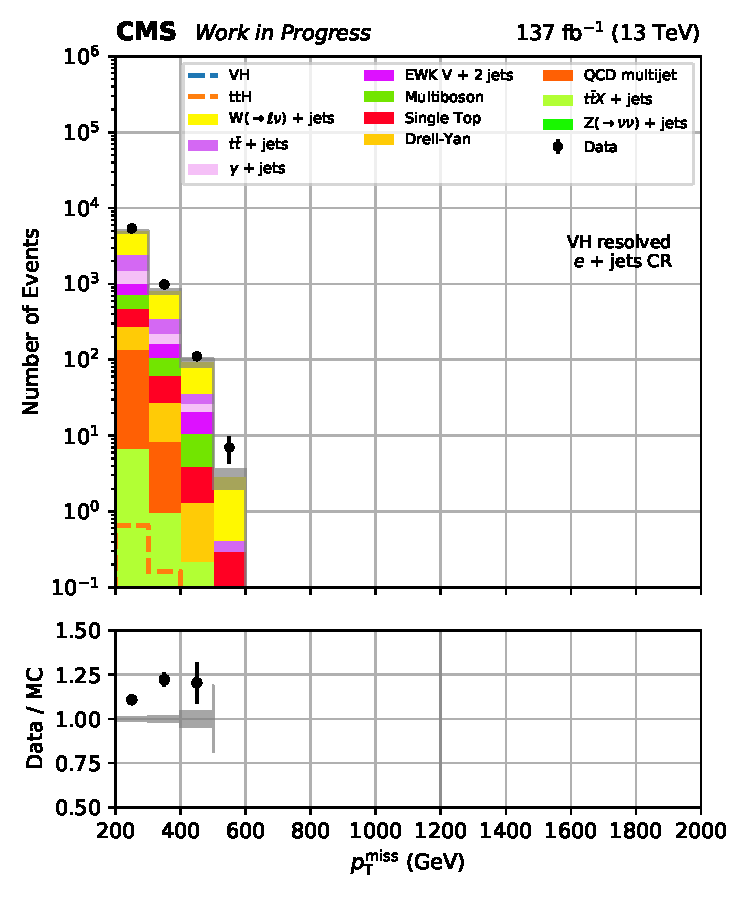
\includegraphics[width=\textwidth]{figures/region_plots/full_Run2/region_3/VH_resolved.pdf}
        \caption{\VH resolved}
    \end{subfigure}
    \caption[Data-simulation comparisons of the \ptmiss distribution in the \singleEleCr control region for the combined boosted and resolved categories for the \ttH and \VH processes, using the full Run-2 dataset]{Data-simulation comparisons of the \ptmiss distribution in the \singleEleCr \gls{CR} for the combined boosted and resolved categories for the \ttH and \VH processes, using the full Run-2 dataset.}
    \label{fig:htoinv_cr_yields_comb2016to18_single_electron}
\end{figure}

\begin{figure}[htbp]
    \centering
    \begin{subfigure}[b]{0.24\textwidth}
        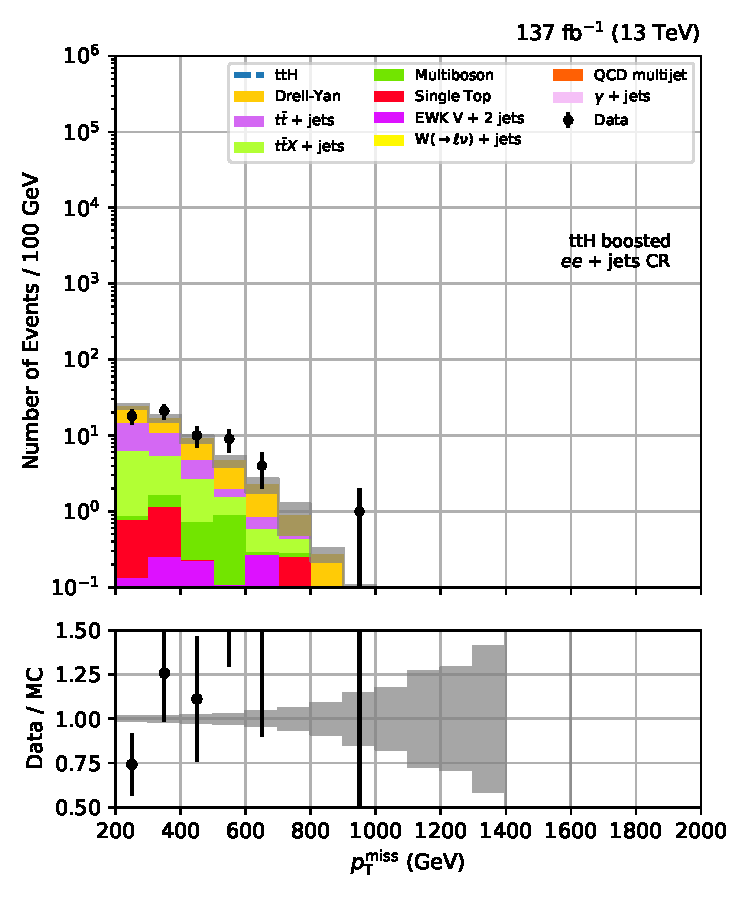
\includegraphics[width=\textwidth]{figures/region_plots/full_Run2/region_4/ttH_boosted.pdf}
        \caption{\ttH boosted}
    \end{subfigure}
    \hfill
    \begin{subfigure}[b]{0.24\textwidth}
        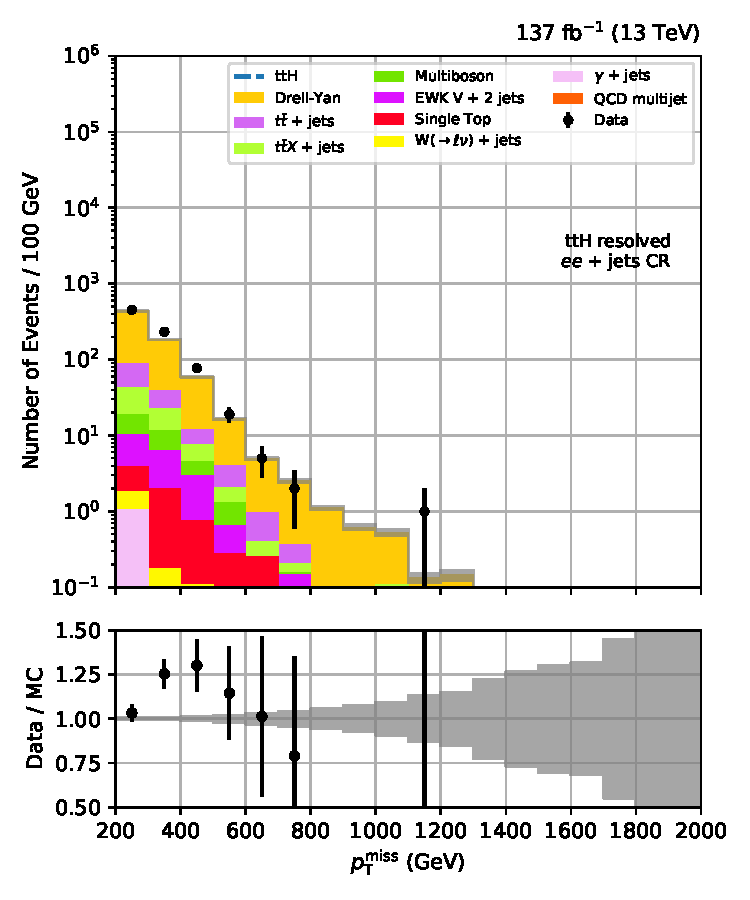
\includegraphics[width=\textwidth]{figures/region_plots/full_Run2/region_4/ttH_resolved.pdf}
        \caption{\ttH resolved}
    \end{subfigure}
    \hfill
    \begin{subfigure}[b]{0.24\textwidth}
        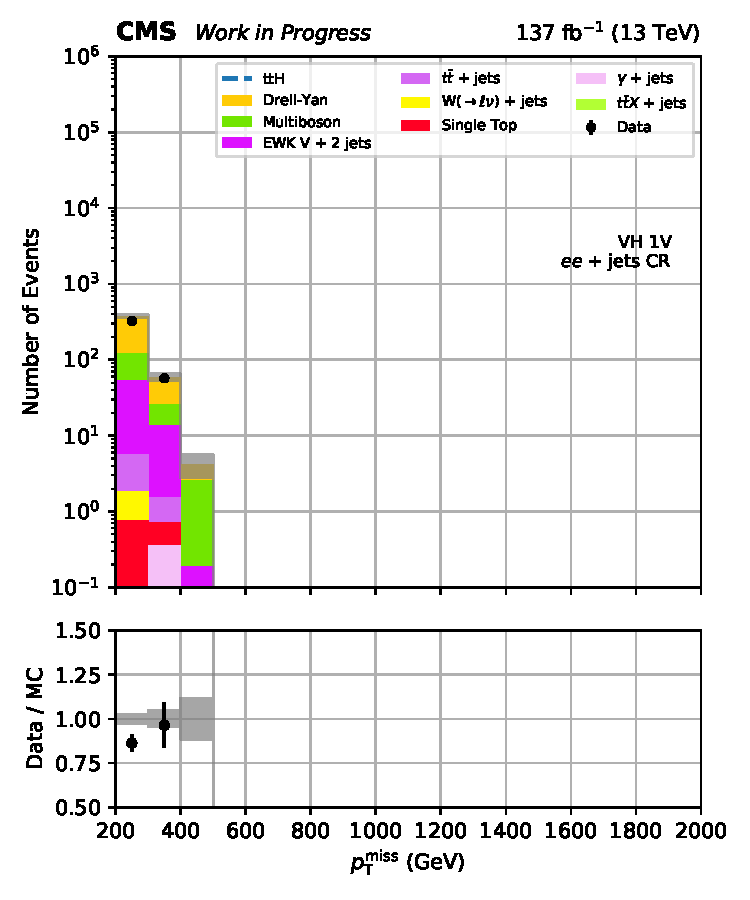
\includegraphics[width=\textwidth]{figures/region_plots/full_Run2/region_4/VH_1V.pdf}
        \caption{\VH 1V}
    \end{subfigure}
    \hfill
    \begin{subfigure}[b]{0.24\textwidth}
        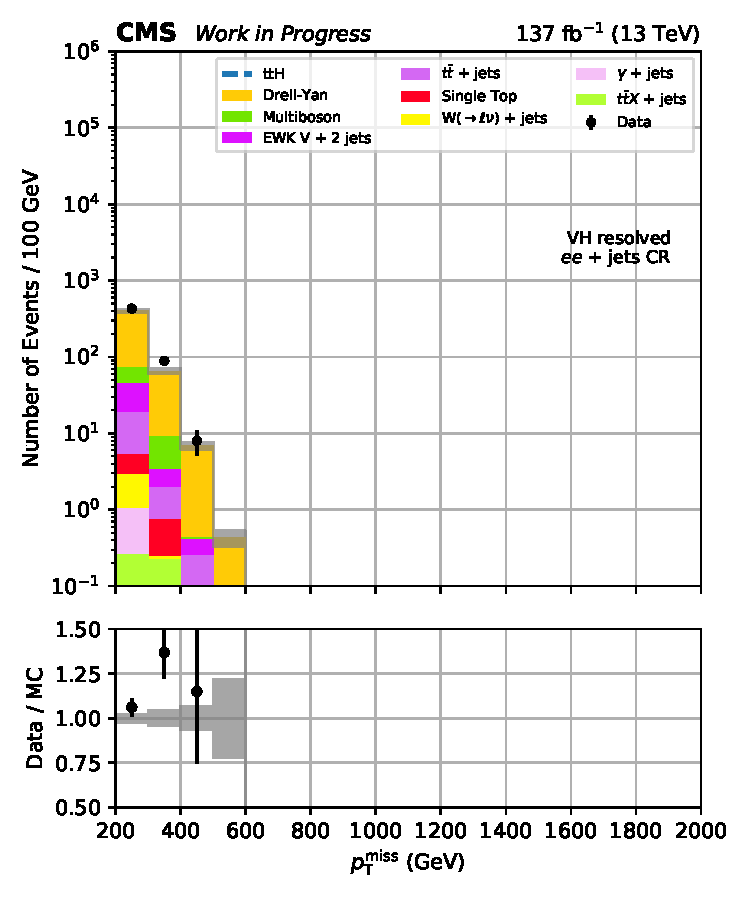
\includegraphics[width=\textwidth]{figures/region_plots/full_Run2/region_4/VH_resolved.pdf}
        \caption{\VH resolved}
    \end{subfigure}
    \caption[Data-simulation comparisons of the \ptmiss distribution in the \doubleEleCr control region for the combined boosted and resolved categories for the \ttH and \VH processes, using the full Run-2 dataset]{Data-simulation comparisons of the \ptmiss distribution in the \doubleEleCr \gls{CR} for the combined boosted and resolved categories for the \ttH and \VH processes, using the full Run-2 dataset.}
    \label{fig:htoinv_cr_yields_comb2016to18_double_electron}
\end{figure}

\begin{figure}[htbp]
    \centering
    \begin{subfigure}[b]{0.24\textwidth}
        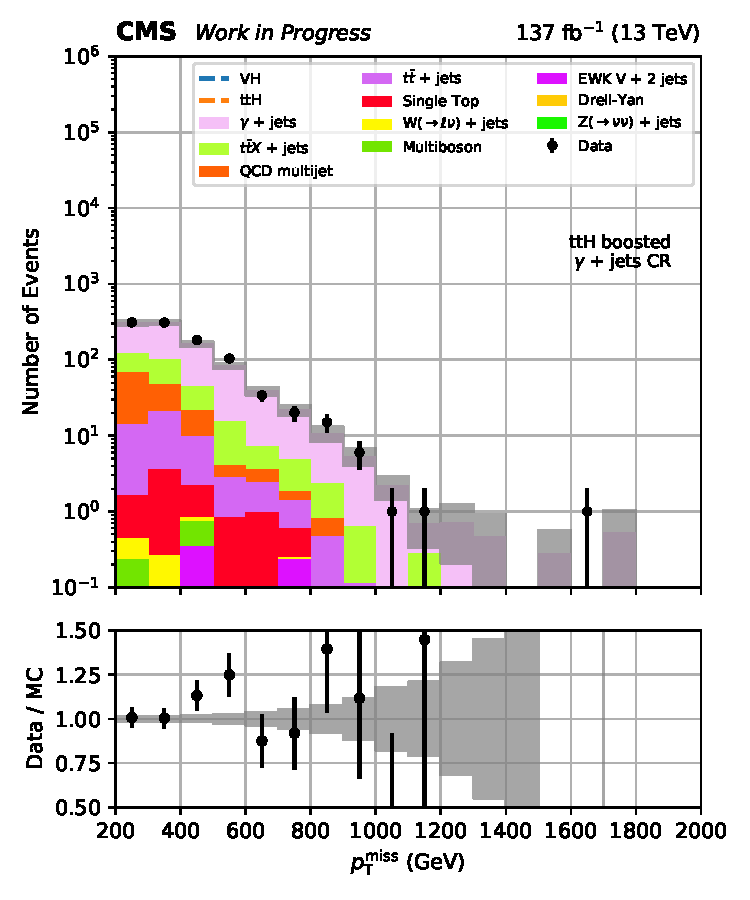
\includegraphics[width=\textwidth]{figures/region_plots/full_Run2/region_5/ttH_boosted.pdf}
        \caption{\ttH boosted}
    \end{subfigure}
    \hfill
    \begin{subfigure}[b]{0.24\textwidth}
        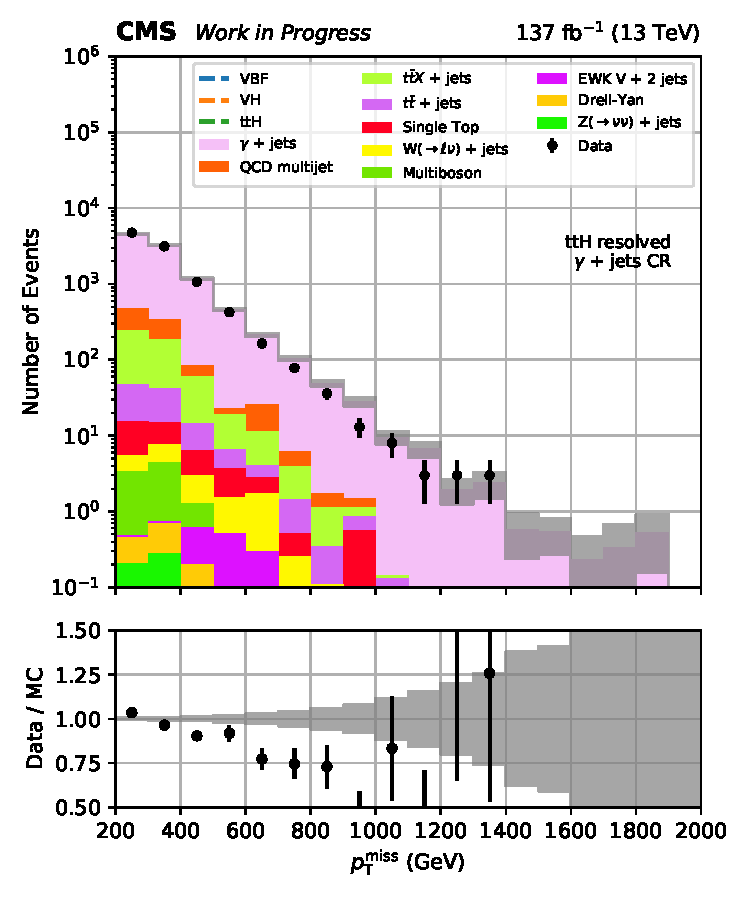
\includegraphics[width=\textwidth]{figures/region_plots/full_Run2/region_5/ttH_resolved.pdf}
        \caption{\ttH resolved}
    \end{subfigure}
    \hfill
    \begin{subfigure}[b]{0.24\textwidth}
        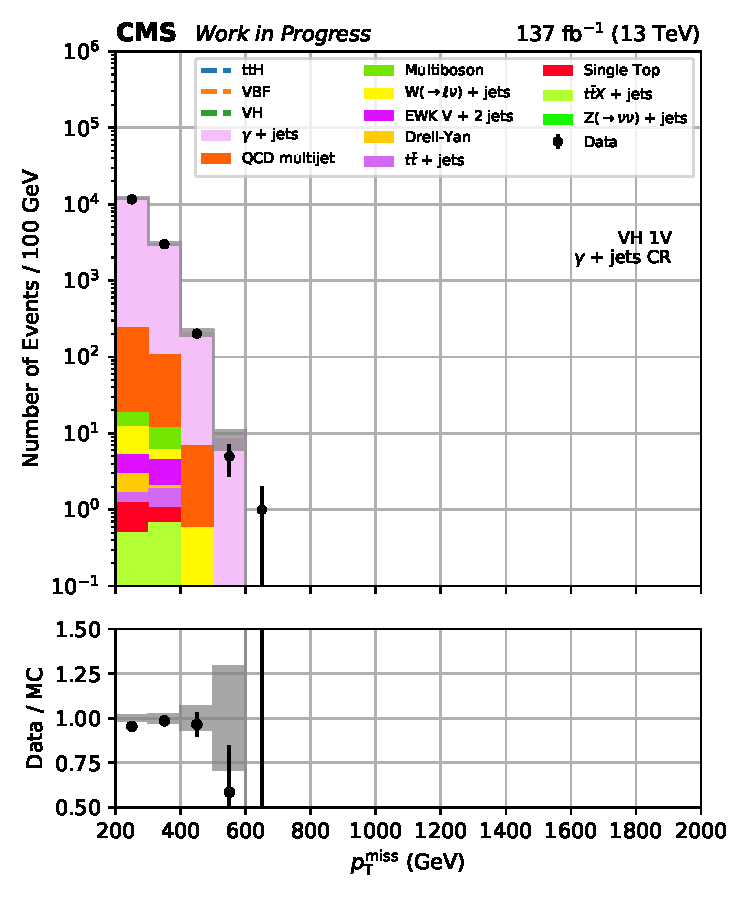
\includegraphics[width=\textwidth]{figures/region_plots/full_Run2/region_5/VH_1V.pdf}
        \caption{\VH 1V}
    \end{subfigure}
    \hfill
    \begin{subfigure}[b]{0.24\textwidth}
        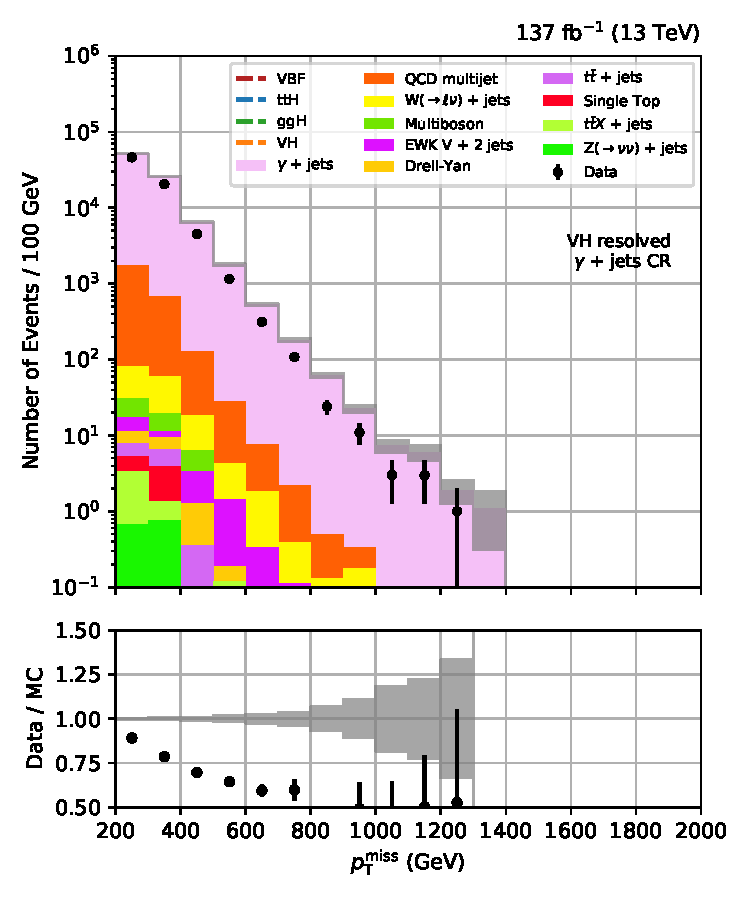
\includegraphics[width=\textwidth]{figures/region_plots/full_Run2/region_5/VH_resolved.pdf}
        \caption{\VH resolved}
    \end{subfigure}
    \caption[Data-simulation comparisons of the \ptmiss distribution in the \singlePhotonCr control region for the combined boosted and resolved categories for the \ttH and \VH processes, using the full Run-2 dataset]{Data-simulation comparisons of the \ptmiss distribution in the \singlePhotonCr \gls{CR} for the combined boosted and resolved categories for the \ttH and \VH processes, using the full Run-2 dataset. Contributions from the \acrshort{qcd} multijet process use the prediction from the photon purity measurement in Chpt.~\ref{subsubsec:htoinv_photon_purity} instead of the \acrshort{mc}.}
    \label{fig:htoinv_cr_yields_comb2016to18_single_photon}
\end{figure}

% Figures from 2nd September, 2020


%=========================================================


\subsubsection{Photon purity measurement for the \texorpdfstring{\singlePhotonCr}{photon} control region}
\label{subsubsec:htoinv_photon_purity}

Photons are reconstructed from clusters in the \acrshort{ecal}. They can usually be discriminated from other sources leaving \acrshort{ecal} deposits due to the properties of the deposits themselves, as well as the lack of other signatures that typically belong to other particles. However, this method is imperfect, and occasionally other particles will incorrectly be identified as photons (known as \emph{fakes}). The leading sources of fake photons is from \acrshort{qcd} multijet events where a \gls{jet} is misidentified as such. Due to the high cross section of the process, even a small rate of fake photons becomes important to consider.

In order to separate real photons from fakes in the \singlePhotonCr \gls{CR}, a purity measurement is performed. We define the purity as the fraction of reconstructed photons that are from an isolated photon emerging from the hard scatter of the event, rather than a fake. The variable $\sieie$ is able to distinguish between real and fake photons with sufficient power. A peak with a hard cut off at $\sieie \approx \text{0.01}$ is observed for real photons, while fakes possess a less pronounced peak and much slower decline above that threshold. As such, we perform a template fit to the distribution in data to extract the purity.

As inputs to the fit, we select photons in data by applying the medium identification requirements in Tab.~\ref{tab:htoinv_photon_ID_barrel} with the exception of $\sieie$ to observe the full range. Photons from \singlePhotonCr simulation are selected with the same criteria and are used to define the real photon template. A fake photon template is obtained from data by requiring at least one of the isolation criteria from the medium ID in Tab.~\ref{tab:htoinv_photon_ID_barrel} to be unfulfilled. This ensures the photons from this set do not overlap with the real photons from data.

The templates are derived in separate bins of photon \pt, and the purity measurement is performed separately for each data taking year. The following event selection is applied:

\medskip
\begin{easylist}[itemize]
    \cutflowlistprops
    & Photon trigger requirement for the respective dataset from Tab.~\ref{tab:htoinv_photon_pd_triggers}
    & \ptmiss filters from Chpt.~\ref{subsec:htoinv_other_filters}
    & $\ptmiss < \text{60}\GeV$
    & At least one jet with $\pt > \text{80}\GeV$ and $\abseta < \text{2.4}$ that is separated from any photon with $\Delta R > \text{0.4}$
    & If a second jet is present, it is required to have $\pt > \text{40}\GeV$ and $\abseta < \text{2.4}$, also separated from any photon with $\Delta R > \text{0.4}$
    & $\HT > \text{200} \GeV$
\end{easylist}

\medskip

\noindent{}A combination of cuts are used to select photons appropriately and ensure the phase space resembles that of the \singlePhotonCr \gls{CR}. The shapes of the real and fake templates are fit to the data using a likelihood function in the range $\text{0.004} \leq \sieie \leq \text{0.02}$. By calculating the purity within acceptance (i.e., $\sieie \leq \text{0.01}$ as given by the medium ID requirement), the \emph{impurity} can be derived as a function of photon \pt. An exponential function is fitted to interpolate within the range that also serves to extrapolate above it. Fig.~\ref{fig:htoinv_photon_impurity} illustrates the impurity vs photon \pt for each data taking year. A 25\,\% uncertainty around the fit is assumed to account for effects related to the binning of the \sieie distribution.

\begin{figure}[htbp]
    \centering
    \begin{subfigure}[b]{0.32\textwidth}
        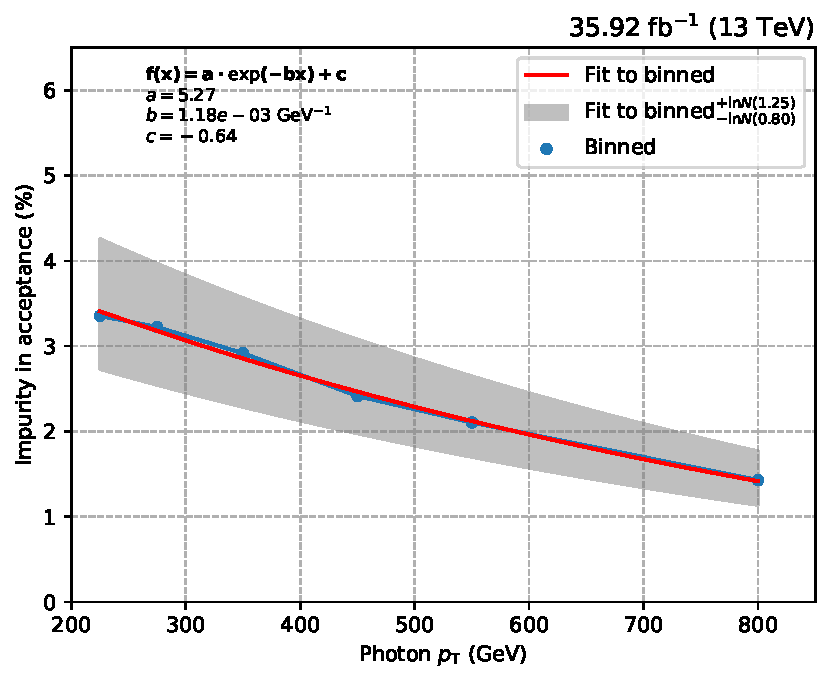
\includegraphics[width=\textwidth]{figures/photon_purity/2016/impurity_plot_2016.pdf}
        \caption{2016}
    \end{subfigure}
    \hfill
    \begin{subfigure}[b]{0.32\textwidth}
        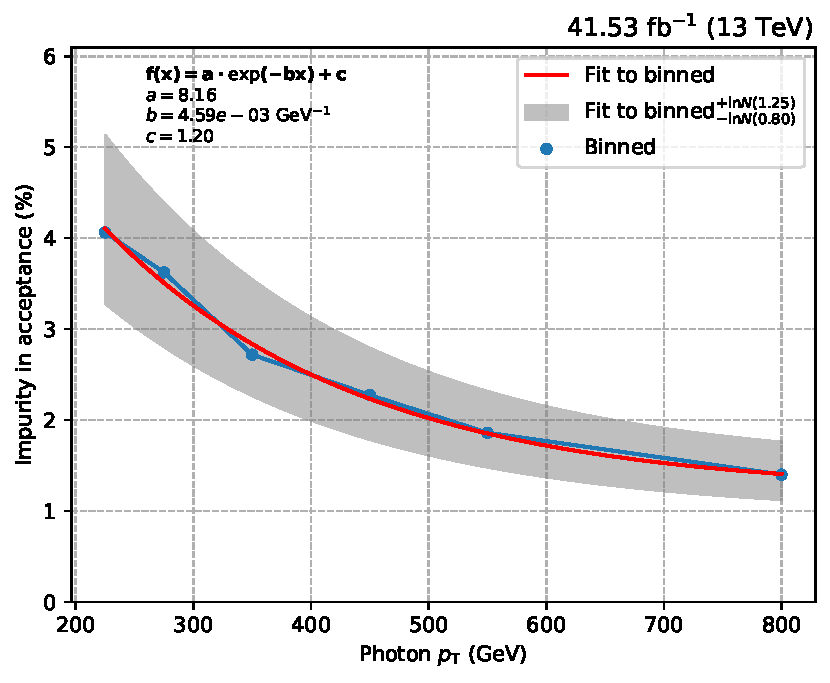
\includegraphics[width=\textwidth]{figures/photon_purity/2017/impurity_plot_2017.pdf}
        \caption{2017}
    \end{subfigure}
    \hfill
    \begin{subfigure}[b]{0.32\textwidth}
        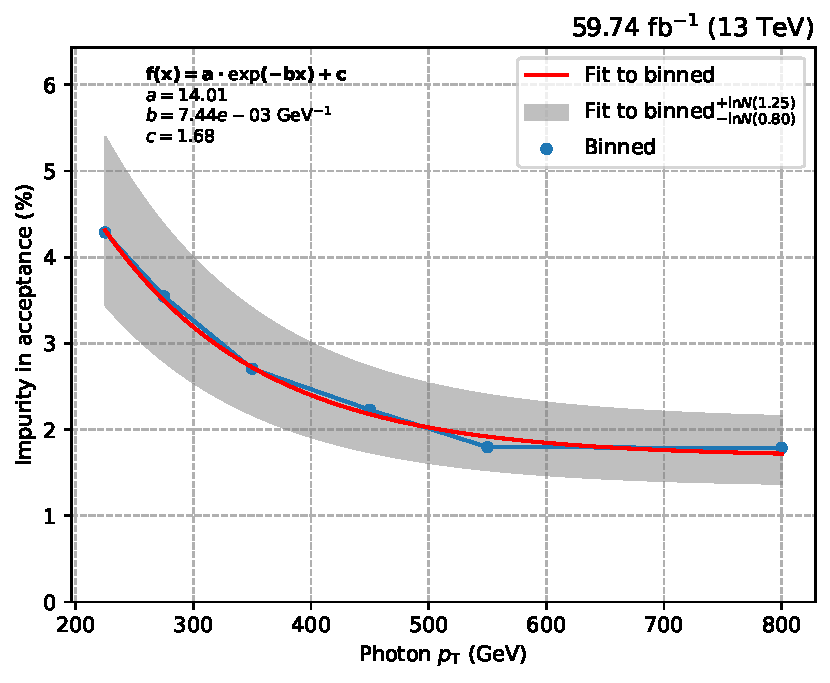
\includegraphics[width=\textwidth]{figures/photon_purity/2018/impurity_plot_2018.pdf}
        \caption{2018}
    \end{subfigure}
    \caption[The fraction of impure photons in data as a function of \pt for each data taking year in Run-2]{The fraction of impure photons in data as a function of \pt for each data taking year in Run-2. An exponential is fit to the binned data with a 25\,\% uncertainty assigned to account for binning effects.}
    \label{fig:htoinv_photon_impurity}
\end{figure}

% Plots from 4th August, 2020

In the analysis, the purity measurement is used to estimate the \acrshort{qcd} multijet background in the \singlePhotonCr \gls{CR}, replacing the contribution from \acrshort{mc}. For each event in data that enters the region, a \acrshort{qcd} multijet pseudo-event is created with the same properties---notably \ptmiss and photon \pt. The value of the impurity calculated from the photon's \pt weights the event. The new \acrshort{qcd} background is therefore generated with the same shape as the data and weighted to represent the rate of non-prompt photons. A 25\,\% uncertainty is attributed to the normalisation of the yield.

% Consider adding a plot or two of data with fit and templates overlaid
% See https://root.cern/doc/master/classTFractionFitter.html for implementation


%=========================================================


\subsection{Sidebands to the signal region}
\label{subsec:htoinv_sidebands}

As explained in Chpt.~\ref{subsec:htoinv_background}, it is difficult to accurately estimate the \acrshort{qcd} multijet content in the signal region. Several kinematic cuts in the analysis are designed to reject \acrshort{qcd} in the signal region, so by inverting one or two of them, we can construct multijet-enriched regions: \emph{\glspl{SB}}.

We invert the requirements on the two angular variables designed to reject multijet events and optimise the categorisation of the production modes (see Chpt.~\ref{subsec:htoinv_cat_optimisation}). Several \glspl{SB} are constructed where each cut is inverted separately, and also when both are inverted. When the angular cut is inverted, the remaining phase space may be split into two \glspl{SB}, dubbed \emph{loose} and \emph{tight}. These are summarised in Tab.~\ref{tab:sideband_defs}.

\begin{table}[htbp]
    \centering
    \begin{tabular}{c|c|c|c}
        & $\omegaTilde < \text{0.2}$ & $\text{0.2} \leq \omegaTilde \leq \text{0.3}$ & $\omegaTilde > \text{0.3}$ \\\hline
        $\dphiFj > \text{0.5}$ & Tight \omegaTilde SB & Loose \omegaTilde SB & Signal region \\\hline
        $\dphiFj \leq \text{0.5}$ & Tight double SB & Loose double SB & \mindphi SB \\
    \end{tabular}
    \caption[Definitions of the data sidebands used to determine the QCD multijet background in the signal region for all categories in the analysis]{Definitions of the \glspl{SB} (SBs) used to determine the \acrshort{qcd} multijet background in the signal region for all categories in the analysis.}
    \label{tab:sideband_defs}
\end{table}

The \glspl{SB} follow the same categorisation as for the other regions, i.e., Tab.~\ref{tab:htoinv_categories}, and are binned in \ptmiss with the same scheme as the other regions. A \gls{SB} composed of the inversion of only one variable maintains similar kinematic properties to the signal region. When performing analysis while still blind to data in the signal region, inspecting one of these \glspl{SB} is a good indicator of how new cuts or corrections will affect the signal region composition, and compatibility between data and \acrshort{mc}. Like the \glspl{CR}, \glspl{SB} serve a secondary purpose.

Figs.~\ref{fig:htoinv_sb_yields_comb2016to18_tight_double}, \ref{fig:htoinv_sb_yields_comb2016to18_loose_double}, \ref{fig:htoinv_sb_yields_comb2016to18_mht_met}, \ref{fig:htoinv_sb_yields_comb2016to18_tight_minOmegaTilde}, and \ref{fig:htoinv_sb_yields_comb2016to18_loose_minOmegaTilde} illustrate the \ptmiss distributions in each \gls{SB} after the analysis-level selections with the full Run-2 dataset. The combined \ttH and \VH subcategories for boosted and resolved topologies are used to demonstrate the shapes and data--simulation resemblance. Background estimation is performed separately for each year due to the differing running conditions, detector configuration, and the different effects or problems seen in the data.\footnote{Might not need to show all of these plots. They're just here for now, and can be tidied up later. May be worth showing \ggH in the same capacity as the other categories, however.}\footnote{Some of the sidebands are unpopulated for \VH because of the \mindphi cut in scenario 5. Make sure to fix.}

\begin{figure}[htbp]
    \centering
    \begin{subfigure}[b]{0.24\textwidth}
        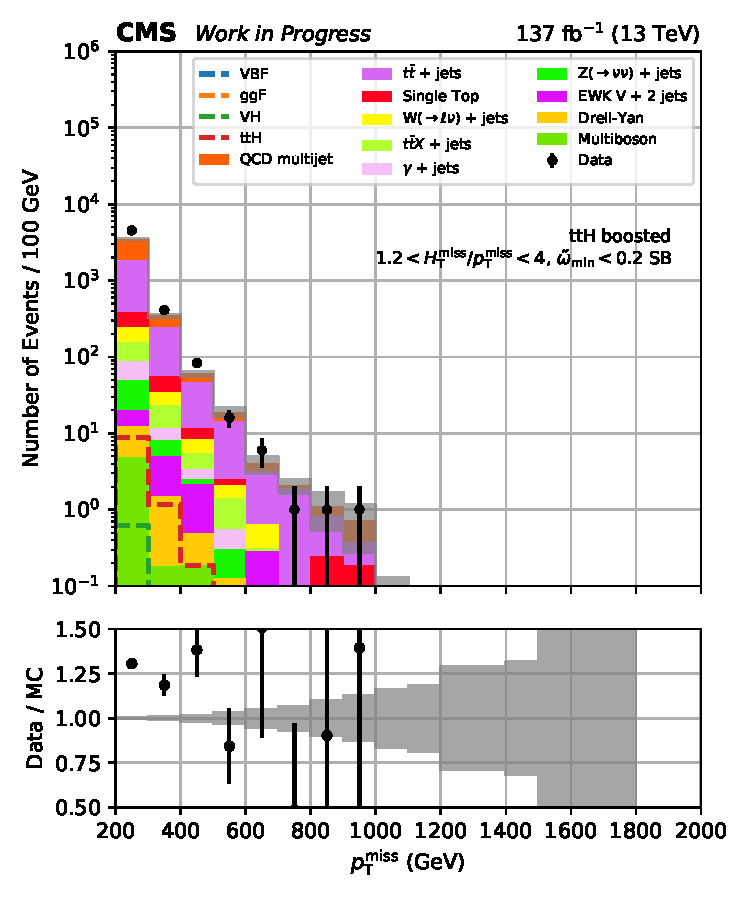
\includegraphics[width=\textwidth]{figures/region_plots/full_Run2/sideband_0/ttH_boosted.pdf}
        \caption{\ttH boosted}
    \end{subfigure}
    \hfill
    \begin{subfigure}[b]{0.24\textwidth}
        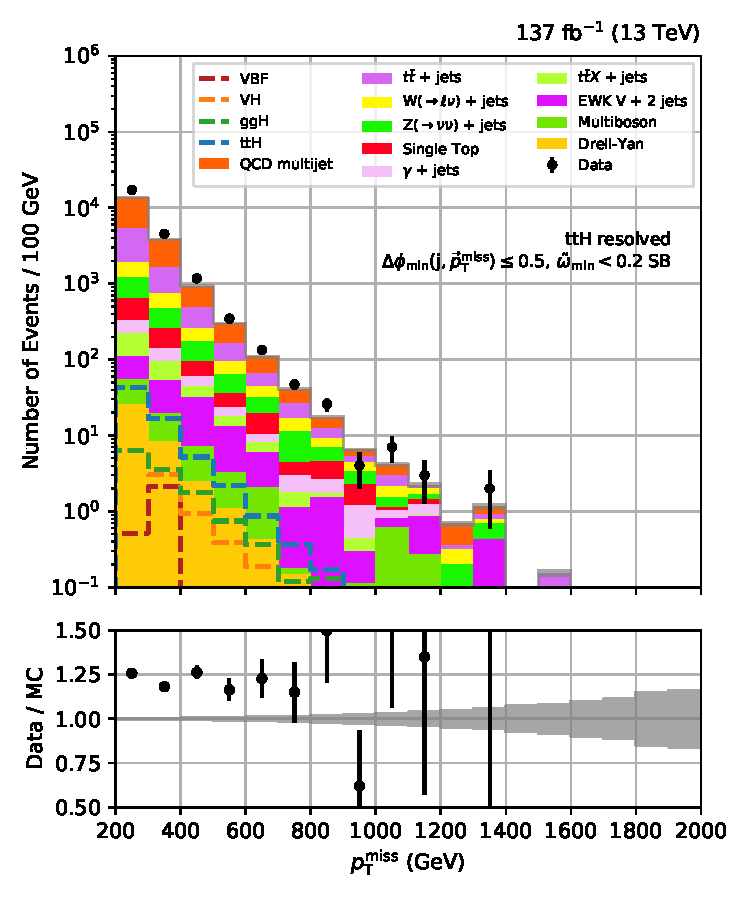
\includegraphics[width=\textwidth]{figures/region_plots/full_Run2/sideband_0/ttH_resolved.pdf}
        \caption{\ttH resolved}
    \end{subfigure}
    \hfill
    \begin{subfigure}[b]{0.24\textwidth}
        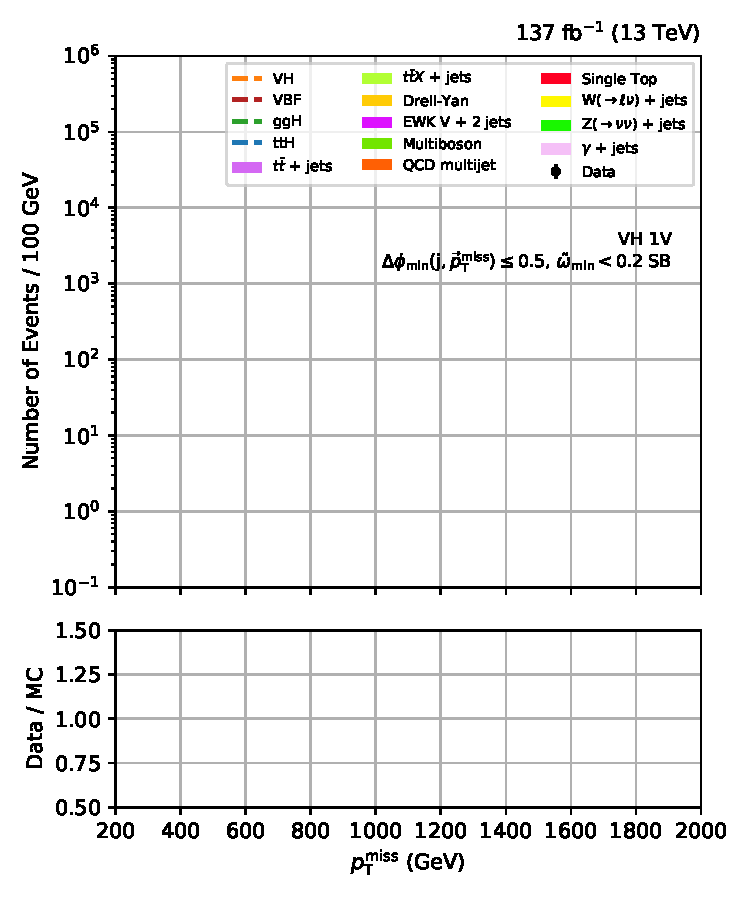
\includegraphics[width=\textwidth]{figures/region_plots/full_Run2/sideband_0/VH_1V.pdf}
        \caption{\VH 1V}
    \end{subfigure}
    \hfill
    \begin{subfigure}[b]{0.24\textwidth}
        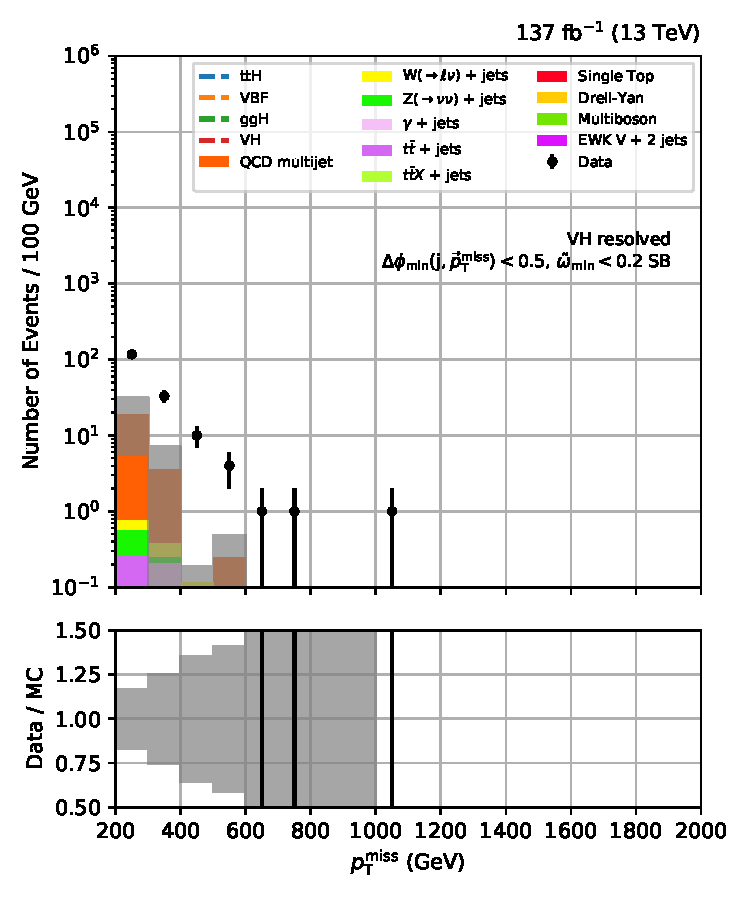
\includegraphics[width=\textwidth]{figures/region_plots/full_Run2/sideband_0/VH_resolved.pdf}
        \caption{\VH resolved}
    \end{subfigure}
    \caption[Data-simulation comparisons of the \ptmiss distribution in the tight double sideband for the combined boosted and resolved categories for the \ttH and \VH processes, using the full Run-2 dataset]{Data-simulation comparisons of the \ptmiss distribution in the tight double \gls{SB} for the combined boosted and resolved categories for the \ttH and \VH processes, using the full Run-2 dataset.}
    \label{fig:htoinv_sb_yields_comb2016to18_tight_double}
\end{figure}

\begin{figure}[htbp]
    \centering
    \begin{subfigure}[b]{0.24\textwidth}
        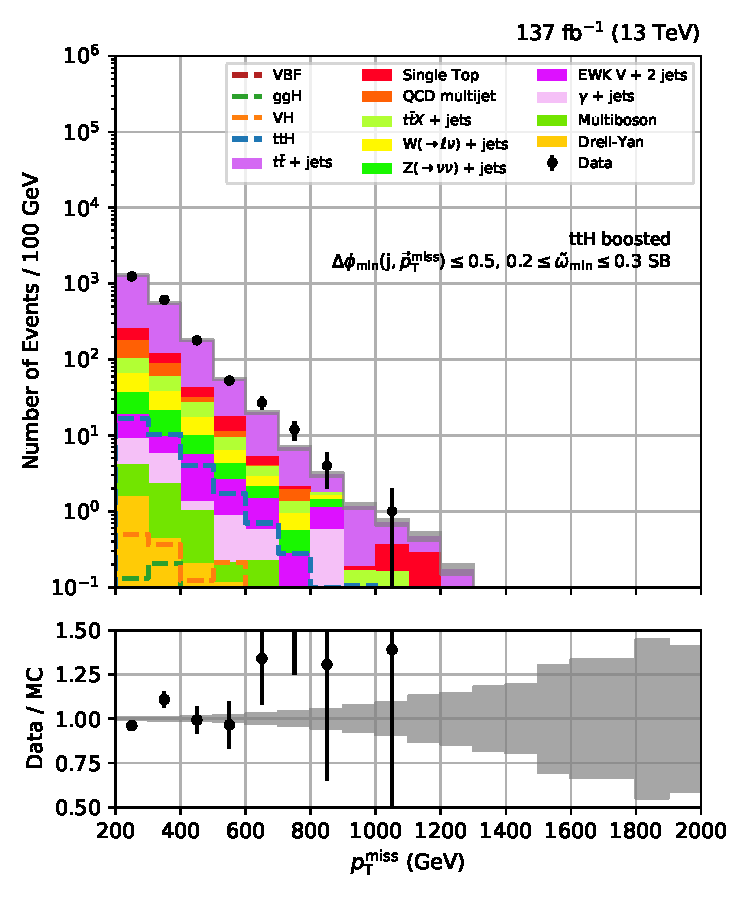
\includegraphics[width=\textwidth]{figures/region_plots/full_Run2/sideband_1/ttH_boosted.pdf}
        \caption{\ttH boosted}
    \end{subfigure}
    \hfill
    \begin{subfigure}[b]{0.24\textwidth}
        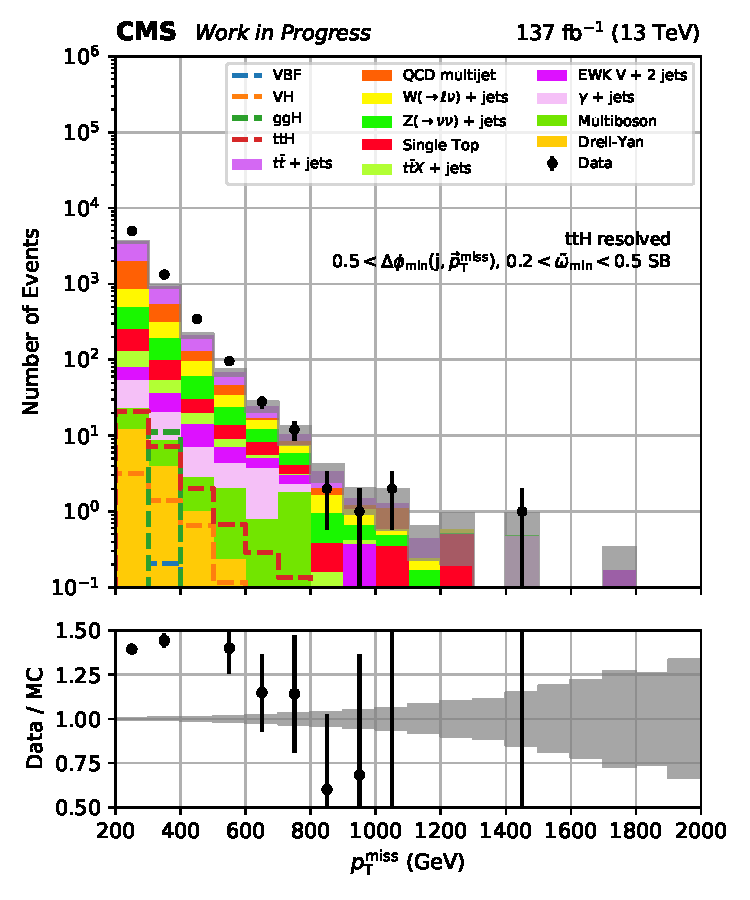
\includegraphics[width=\textwidth]{figures/region_plots/full_Run2/sideband_1/ttH_resolved.pdf}
        \caption{\ttH resolved}
    \end{subfigure}
    \hfill
    \begin{subfigure}[b]{0.24\textwidth}
        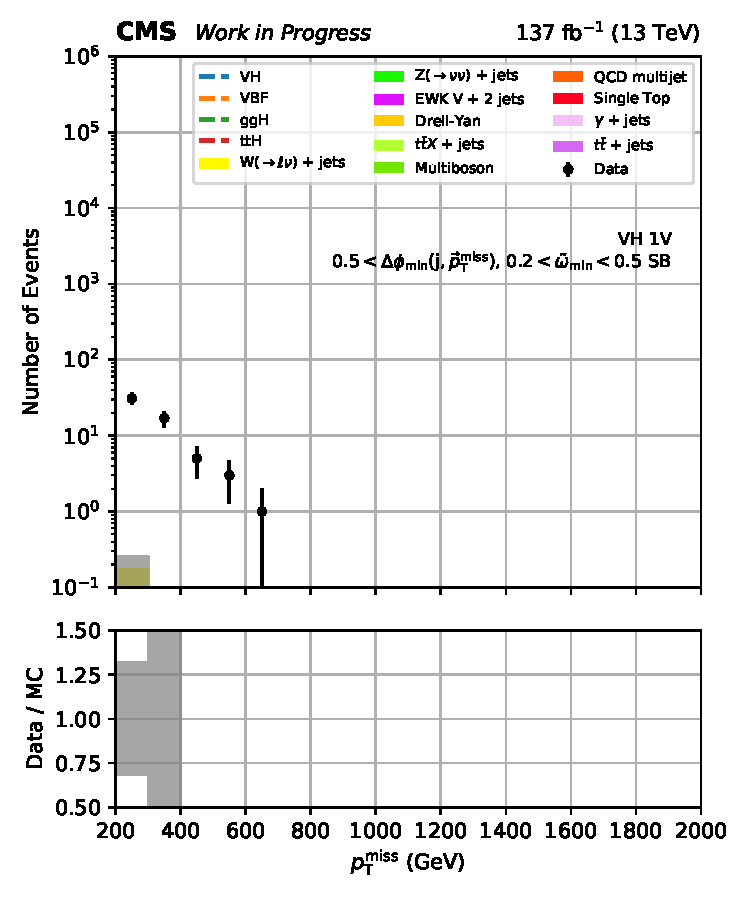
\includegraphics[width=\textwidth]{figures/region_plots/full_Run2/sideband_1/VH_1V.pdf}
        \caption{\VH 1V}
    \end{subfigure}
    \hfill
    \begin{subfigure}[b]{0.24\textwidth}
        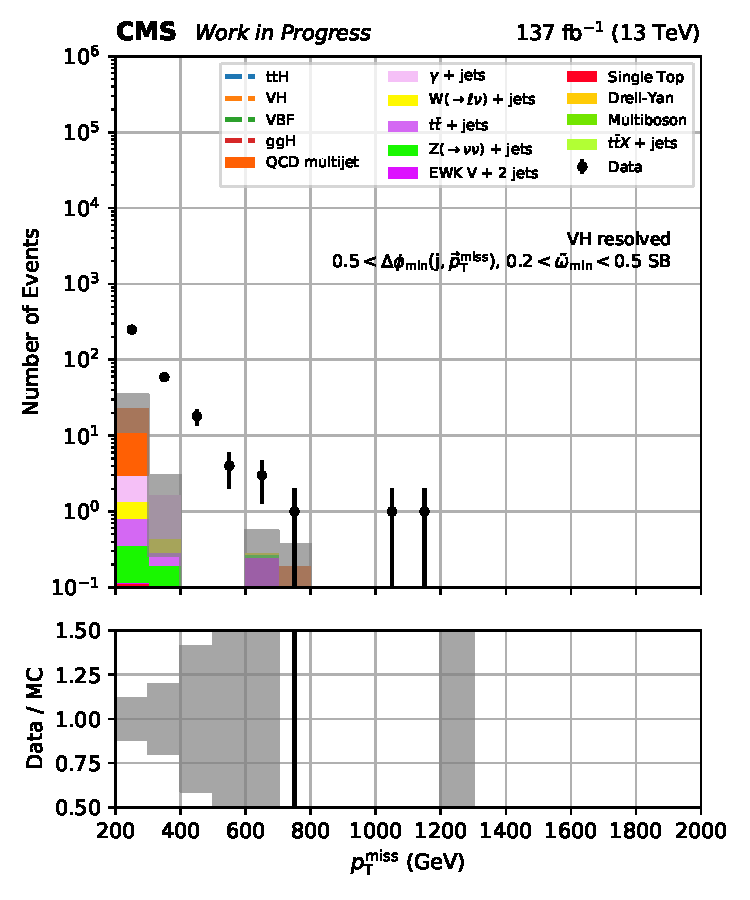
\includegraphics[width=\textwidth]{figures/region_plots/full_Run2/sideband_1/VH_resolved.pdf}
        \caption{\VH resolved}
    \end{subfigure}
    \caption[Data-simulation comparisons of the \ptmiss distribution in the loose double sideband for the combined boosted and resolved categories for the \ttH and \VH processes, using the full Run-2 dataset]{Data-simulation comparisons of the \ptmiss distribution in the loose double \gls{SB} for the combined boosted and resolved categories for the \ttH and \VH processes, using the full Run-2 dataset.}
    \label{fig:htoinv_sb_yields_comb2016to18_loose_double}
\end{figure}
\begin{figure}[htbp]
    \centering
    \begin{subfigure}[b]{0.24\textwidth}
        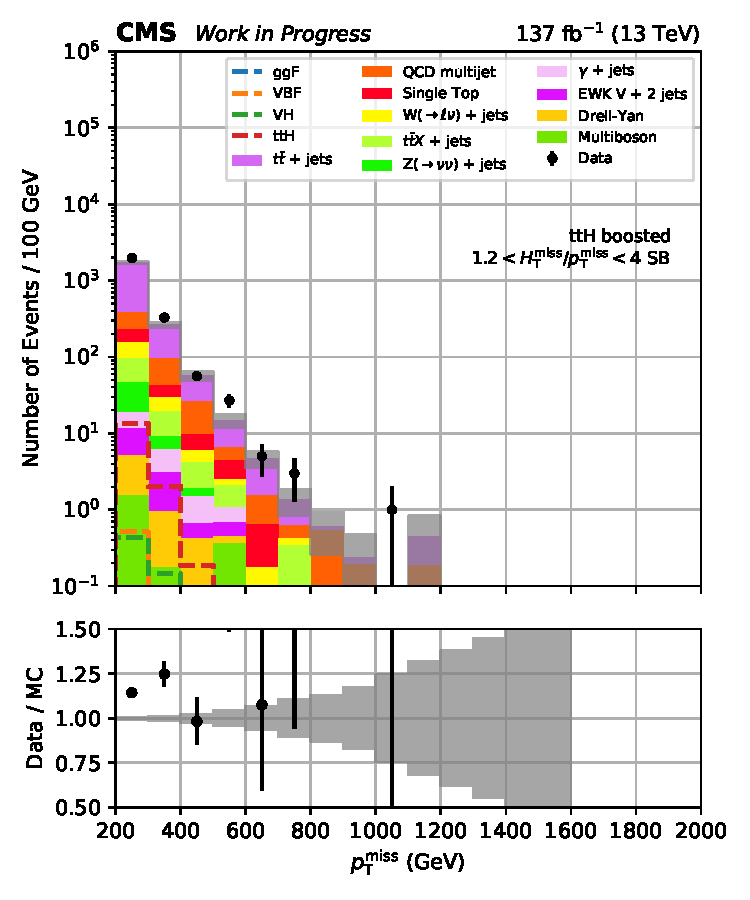
\includegraphics[width=\textwidth]{figures/region_plots/full_Run2/sideband_2/ttH_boosted.pdf}
        \caption{\ttH boosted}
    \end{subfigure}
    \hfill
    \begin{subfigure}[b]{0.24\textwidth}
        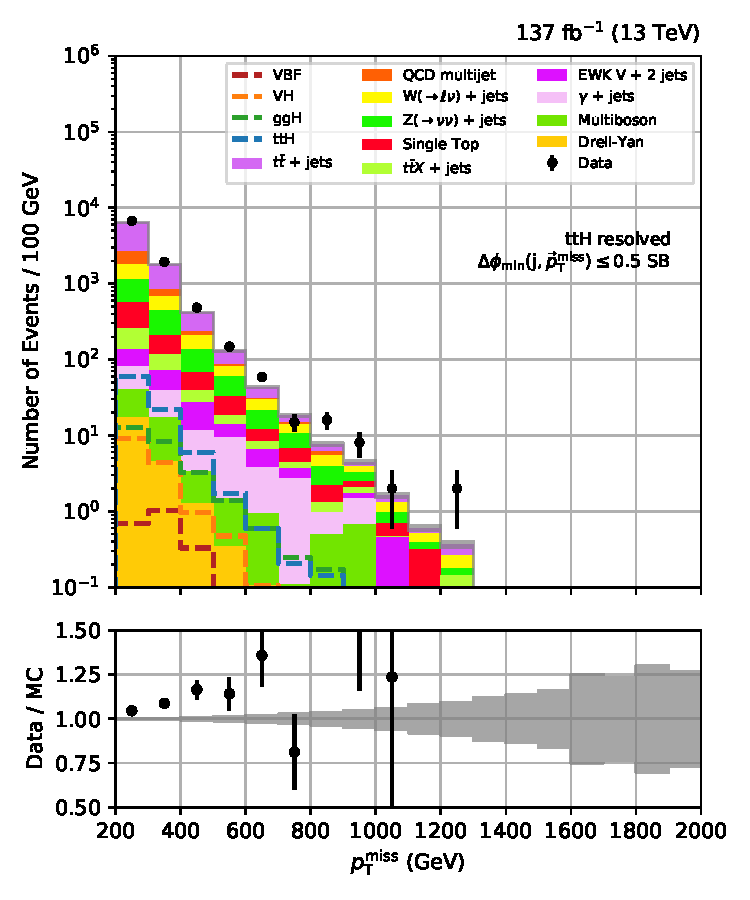
\includegraphics[width=\textwidth]{figures/region_plots/full_Run2/sideband_2/ttH_resolved.pdf}
        \caption{\ttH resolved}
    \end{subfigure}
    \hfill
    \begin{subfigure}[b]{0.24\textwidth}
        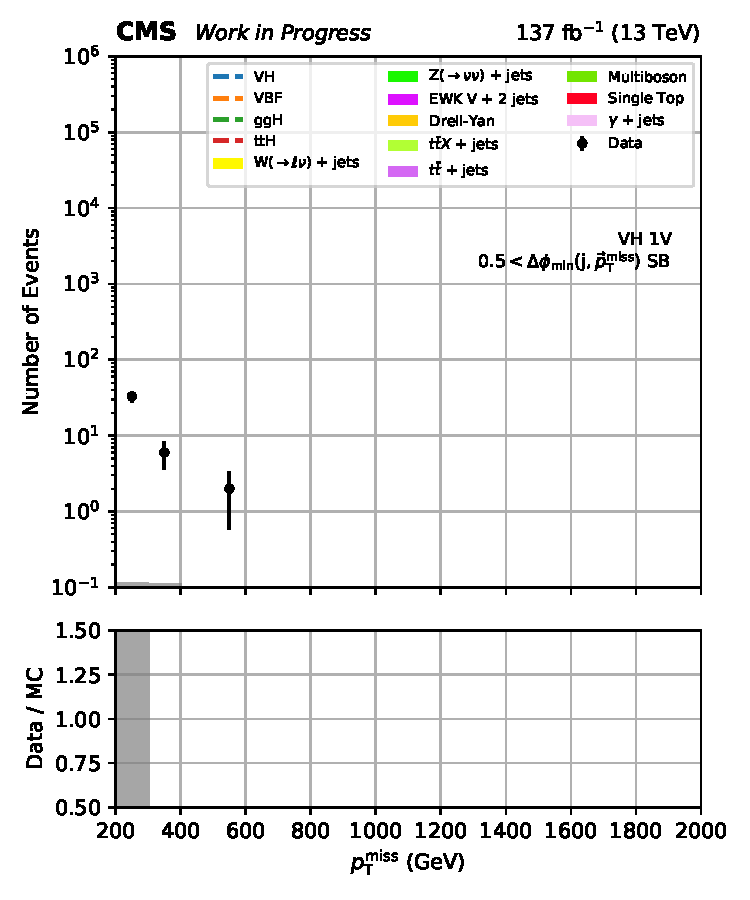
\includegraphics[width=\textwidth]{figures/region_plots/full_Run2/sideband_2/VH_1V.pdf}
        \caption{\VH 1V}
    \end{subfigure}
    \hfill
    \begin{subfigure}[b]{0.24\textwidth}
        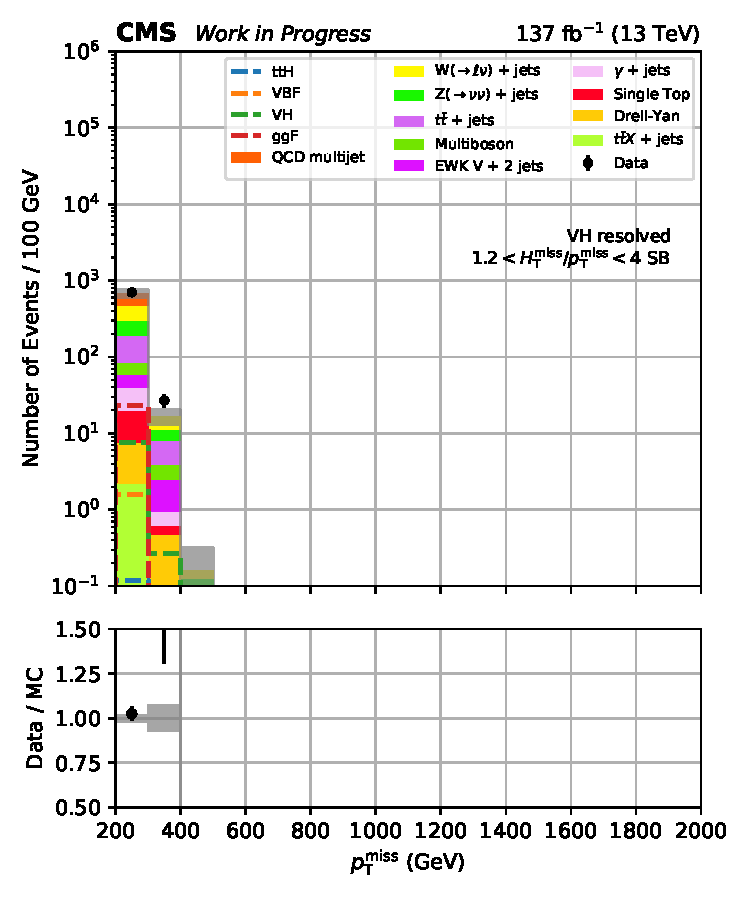
\includegraphics[width=\textwidth]{figures/region_plots/full_Run2/sideband_2/VH_resolved.pdf}
        \caption{\VH resolved}
    \end{subfigure}
    \caption[Data-simulation comparisons of the \ptmiss distribution in the $\mht/\ptmiss$ sideband for the combined boosted and resolved categories for the \ttH and \VH processes, using the full Run-2 dataset]{Data-simulation comparisons of the \ptmiss distribution in the $\mht/\ptmiss$ \gls{SB} for the combined boosted and resolved categories for the \ttH and \VH processes, using the full Run-2 dataset.}
    \label{fig:htoinv_sb_yields_comb2016to18_mht_met}
\end{figure}

\begin{figure}[htbp]
    \centering
    \begin{subfigure}[b]{0.24\textwidth}
        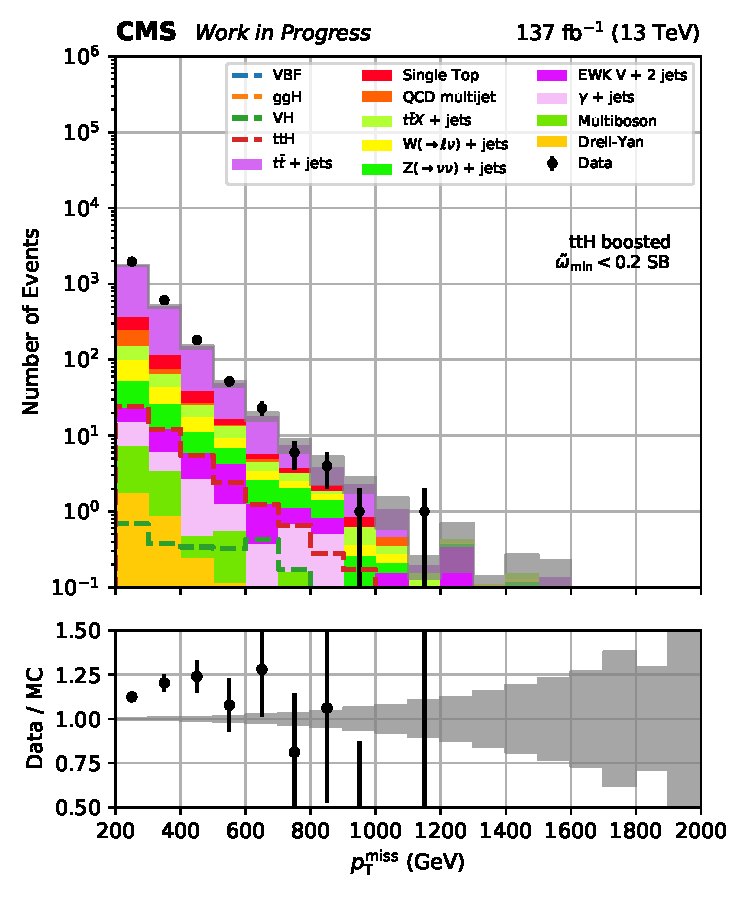
\includegraphics[width=\textwidth]{figures/region_plots/full_Run2/sideband_3/ttH_boosted.pdf}
        \caption{\ttH boosted}
    \end{subfigure}
    \hfill
    \begin{subfigure}[b]{0.24\textwidth}
        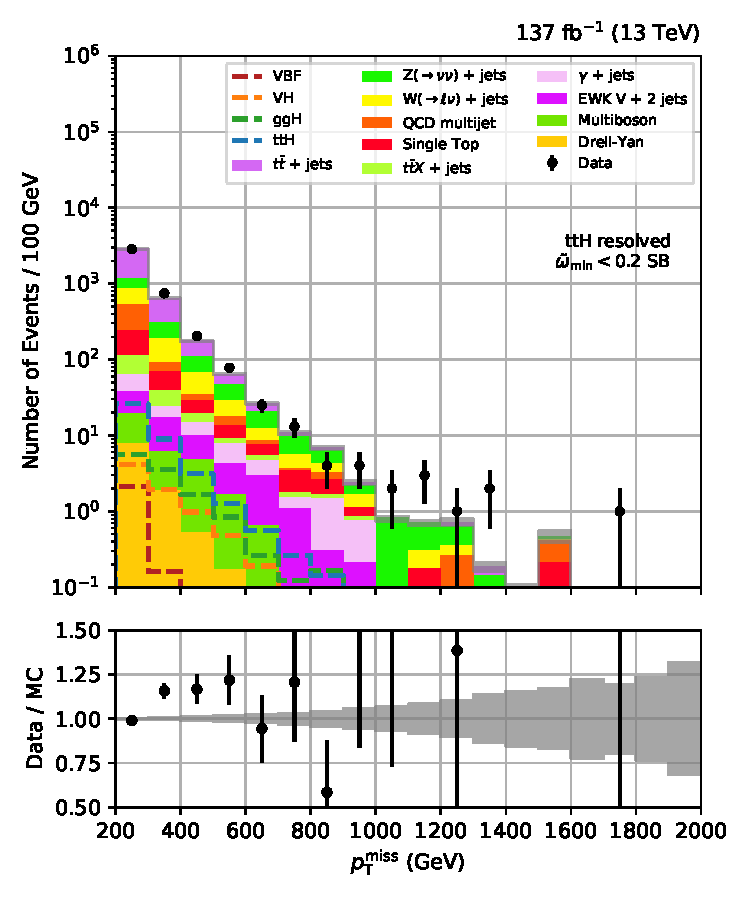
\includegraphics[width=\textwidth]{figures/region_plots/full_Run2/sideband_3/ttH_resolved.pdf}
        \caption{\ttH resolved}
    \end{subfigure}
    \hfill
    \begin{subfigure}[b]{0.24\textwidth}
        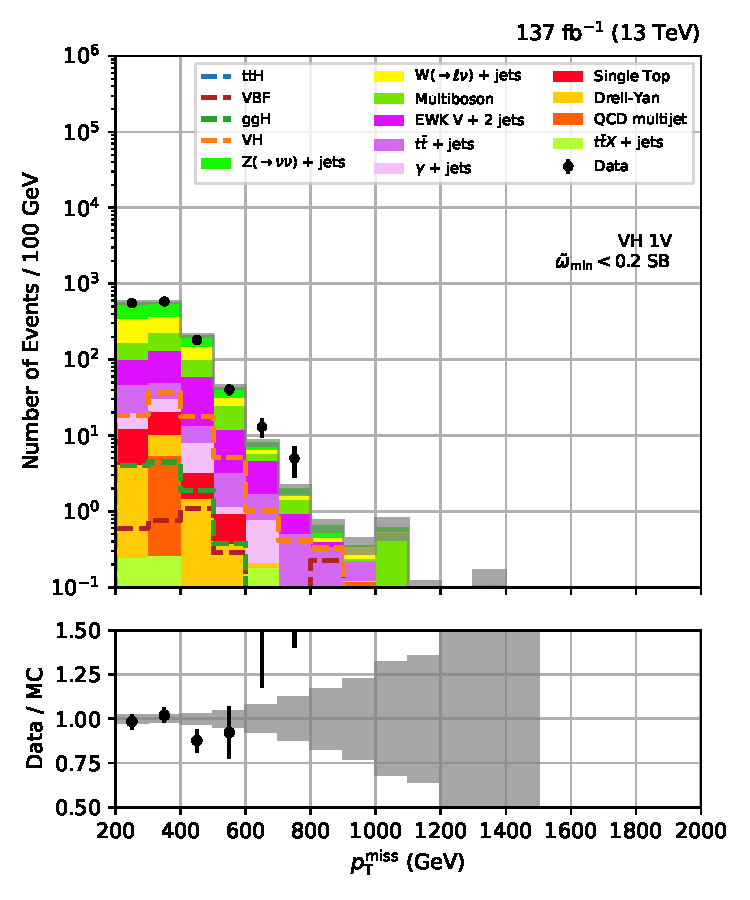
\includegraphics[width=\textwidth]{figures/region_plots/full_Run2/sideband_3/VH_1V.pdf}
        \caption{\VH 1V}
    \end{subfigure}
    \hfill
    \begin{subfigure}[b]{0.24\textwidth}
        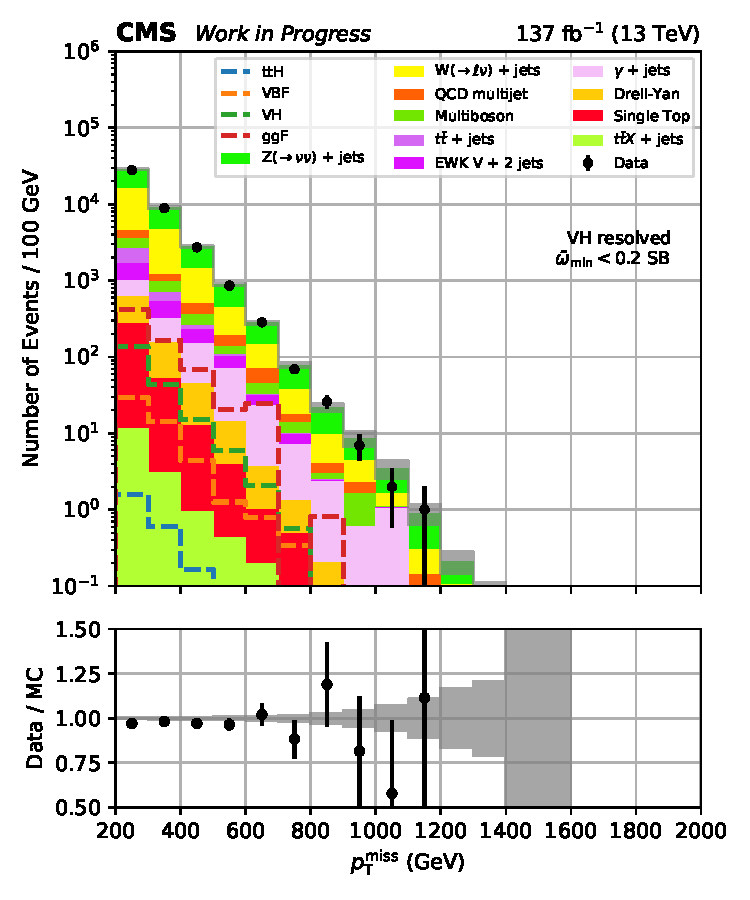
\includegraphics[width=\textwidth]{figures/region_plots/full_Run2/sideband_3/VH_resolved.pdf}
        \caption{\VH resolved}
    \end{subfigure}
    \caption[Data-simulation comparisons of the \ptmiss distribution in the tight \omegaTilde sideband for the combined boosted and resolved categories for the \ttH and \VH processes, using the full Run-2 dataset]{Data-simulation comparisons of the \ptmiss distribution in the tight \omegaTilde \gls{SB} for the combined boosted and resolved categories for the \ttH and \VH processes, using the full Run-2 dataset.}
    \label{fig:htoinv_sb_yields_comb2016to18_tight_minOmegaTilde}
\end{figure}

\begin{figure}[htbp]
    \centering
    \begin{subfigure}[b]{0.24\textwidth}
        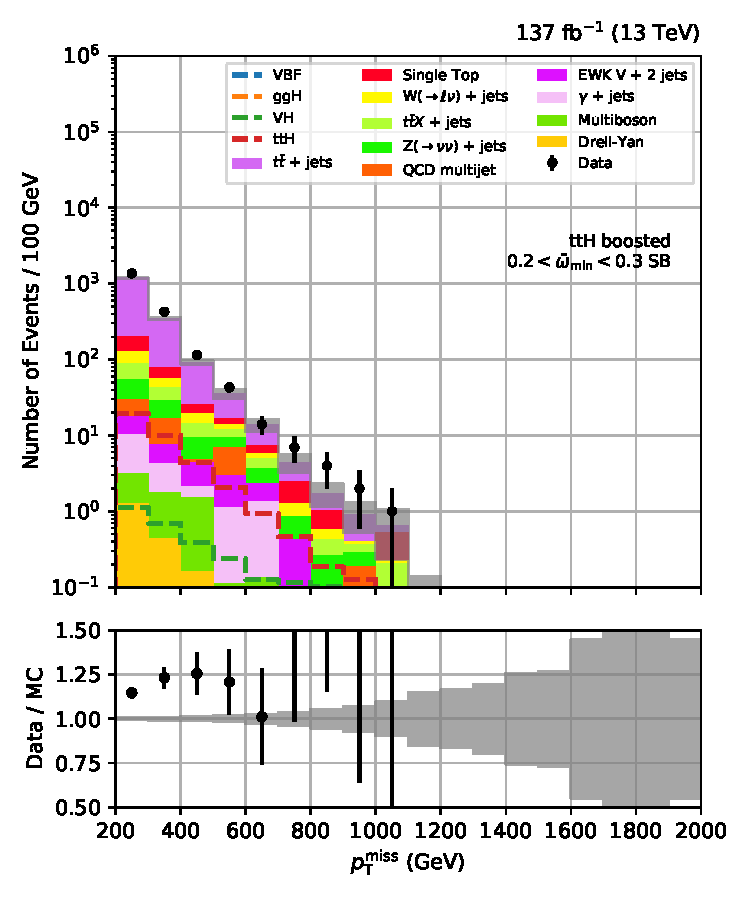
\includegraphics[width=\textwidth]{figures/region_plots/full_Run2/sideband_4/ttH_boosted.pdf}
        \caption{\ttH boosted}
    \end{subfigure}
    \hfill
    \begin{subfigure}[b]{0.24\textwidth}
        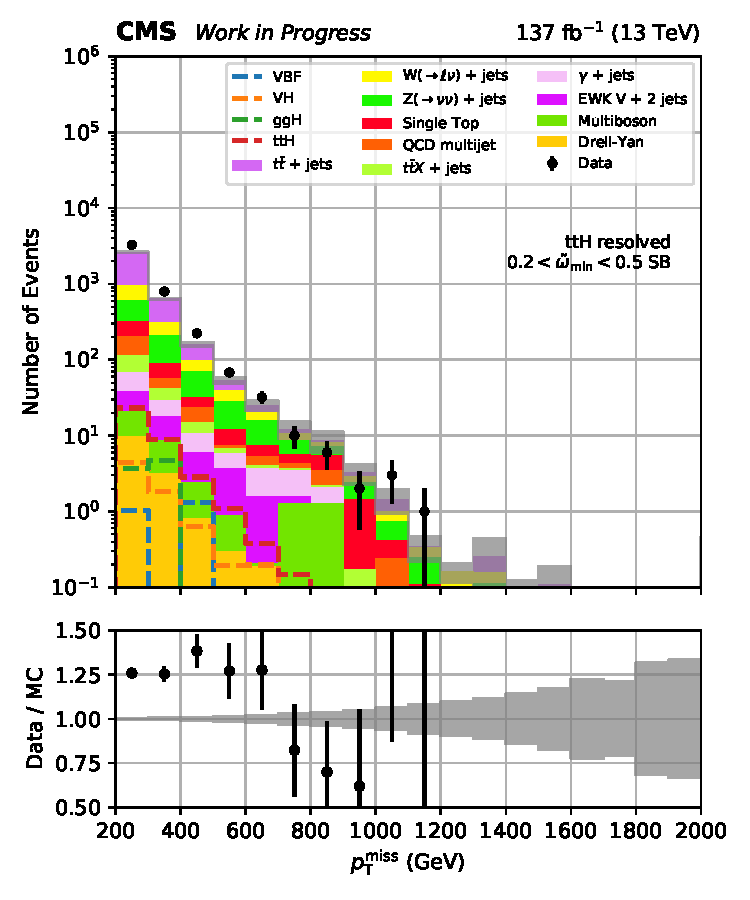
\includegraphics[width=\textwidth]{figures/region_plots/full_Run2/sideband_4/ttH_resolved.pdf}
        \caption{\ttH resolved}
    \end{subfigure}
    \begin{subfigure}[b]{0.24\textwidth}
        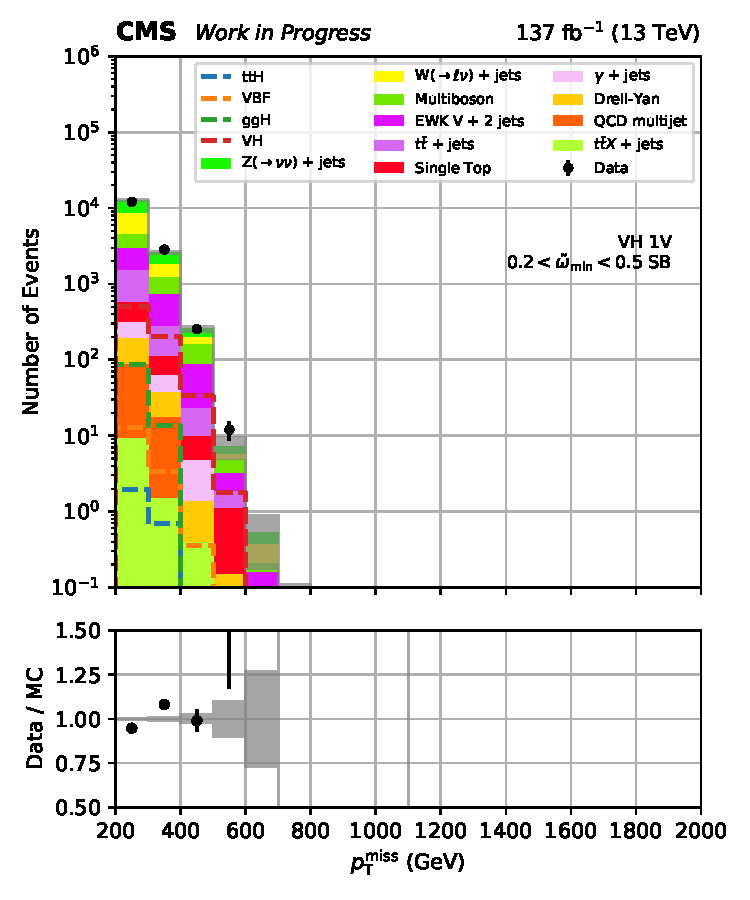
\includegraphics[width=\textwidth]{figures/region_plots/full_Run2/sideband_4/VH_1V.pdf}
        \caption{\VH 1V}
    \end{subfigure}
    \hfill
    \begin{subfigure}[b]{0.24\textwidth}
        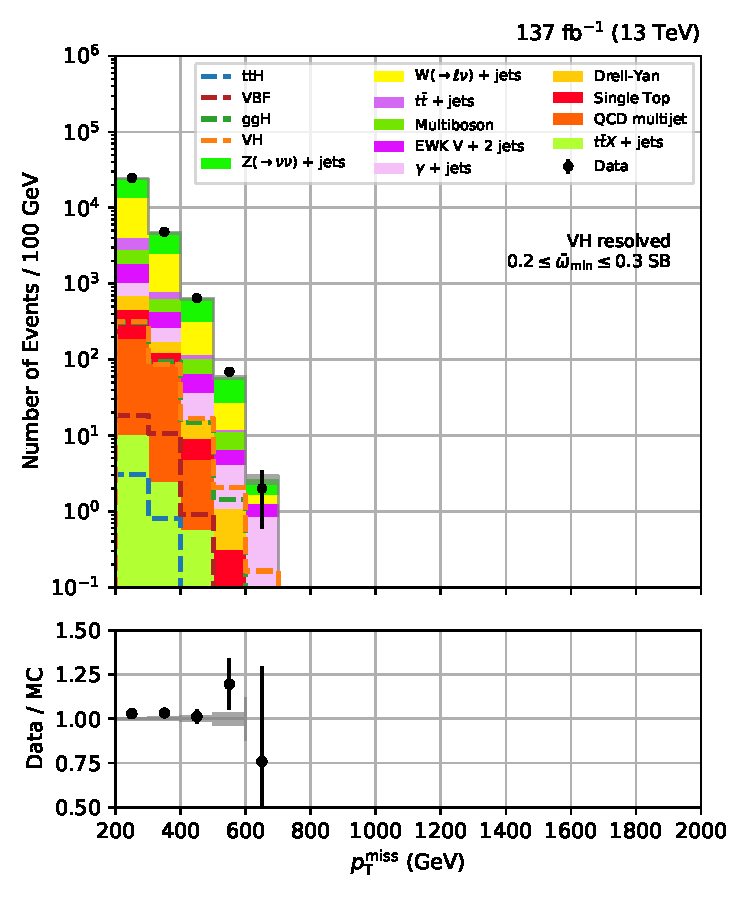
\includegraphics[width=\textwidth]{figures/region_plots/full_Run2/sideband_4/VH_resolved.pdf}
        \caption{\VH resolved}
    \end{subfigure}
    \caption[Data-simulation comparisons of the \ptmiss distribution in the loose \omegaTilde sideband for the combined boosted and resolved categories for the \ttH and \VH processes, using the full Run-2 dataset]{Data-simulation comparisons of the \ptmiss distribution in the loose \omegaTilde \gls{SB} for the combined boosted and resolved categories for the \ttH and \VH processes, using the full Run-2 dataset.}
    \label{fig:htoinv_sb_yields_comb2016to18_loose_minOmegaTilde}
\end{figure}

% Figures from 2nd September, 2020
